\section{Resultados}

\attachfilesetup{
    color = {1 0 0}
} 

\begin{frame}{Implementação dos algoritmos}
    Os algoritmos apresentados foram implementados com a ajuda dos seguintes softwares.
    \vspace{0.5cm}
    
    \begin{itemize}
        \item MATLAB\textregistered \  R2018a
        \item ITA Toolbox (plugin para MATLAB) \cite{ITA_Toolbox}
    \end{itemize}
    \vspace{0.5cm}

    São utilizadas três bases de dados para gerar as RIRSMs e AVCDs.
    \vspace{0.5cm}

    \begin{itemize}
        \item Base de amostras de voz anecóicas
        \item Base de RIRs - Aachen Impulse Response database
        \item Base de ruídos - MUSAN
    \end{itemize}
\end{frame}

\begin{frame}{Implementação dos algoritmos}
    Configurações das características desejadas.
    \vspace{1cm}

    \begin{table} [H]
        \centering
        \begin{tabular}{c|p{7cm}}
    
            \multicolumn{1}{c|}{\textbf{Parâmetro}} & \multicolumn{1}{c}{\textbf{Faixa}} \\
            \hline 
    
            $DRR_{alvo}$ (dB) & $-6 \le DRR_{alvo} \le 18 $ \\
            & \\
            $T60_{alvo}$ (s) & $T60_{org} - 1  \le T60_{alvo} \le T60_{org} + 1$ , onde o limite inferior de $T60_{alvo} = 0.2$ \\
            & \\
            $SNR_{alvo}$ & $3 \le SNR_{alvo} \le 20 $ \\
    
        \end{tabular}
    \end{table}
\end{frame}

%% ---------------------------------------------------------------------------
% RESULTADOS - DRR
\begin{frame}{Resultados - DRR}
    \begin{table} [H]
        \centering
        \label{tbl:da-drr}
        \begin{tabular}{c|c|c|c}
    
            \textbf{Exemplo} & 
            \textbf{Sala RIR} & 
            \textbf{Distância (m)} &
            \textbf{Amostra de Voz} \\
            \hline 
    
            D1 & lecture & 7.1 & H2-T2 \\
            D2 & booth & 1 & H2-T1 \\
            D3 & office & 2 & M2-T2 \\
    
        \end{tabular}
        \bigbreak
        \bigbreak
        \begin{tabular}{c|c|c|c|c}
    
            \textbf{Exemplo} & 
            \textbf{$DRR_{org}$ (dB)} & 
            \textbf{$DRR_{alvo}$ (dB)} &
            \textbf{$DRR_{res}$ (dB)} & 
            \textbf{$\rho_{DRR}$ (\%)} \\
            \hline 
    
            D1 & -4,5 & 10 & 10 & 0 \\
            D2 & 4,7 & -2 & -2 & 0 \\
            D3 & 0,5 & 18 & 18 & 0 \\
    
        \end{tabular}
        \vspace{0.5cm}

        $\rho_{DRR} = |DRR_{res} - DRR_{alvo}|/DRR_{alvo}$
    \end{table}
\end{frame}

\begin{frame}{Resultados - DRR}
    \textbf{Experimento empírico}: sensação subjetiva de “distância”, ordenado de mais para menos distante.
    \vspace{1cm}
    
    \begin{table} [H]
        \centering
        \begin{tabular}{c|c|c|c|c}
    
            \textbf{Exemplo} & 
            \textbf{$DRR_{org}$ (dB)} & 
            \textbf{$DRR_{res}$ (dB)} & 
            \textbf{Comparação} &
            \textbf{Ordem} \\
            \hline 
    
            D1 & -4,5 & 10 & original & 2 \\
            D2 & 4,7 & -2 & simulado & 1 \\
            D3 & 0,5 & 18 & original & 3 \\
    
        \end{tabular}
    \end{table}
\end{frame}

\begin{frame}{Exemplo D1}
    \begin{columns}
        \column{.6\textwidth}
        \begin{figure}
            \begin{subfigure}{\textwidth}
                \centering
                \notextattachfile{\scriptsize RIR Original}
                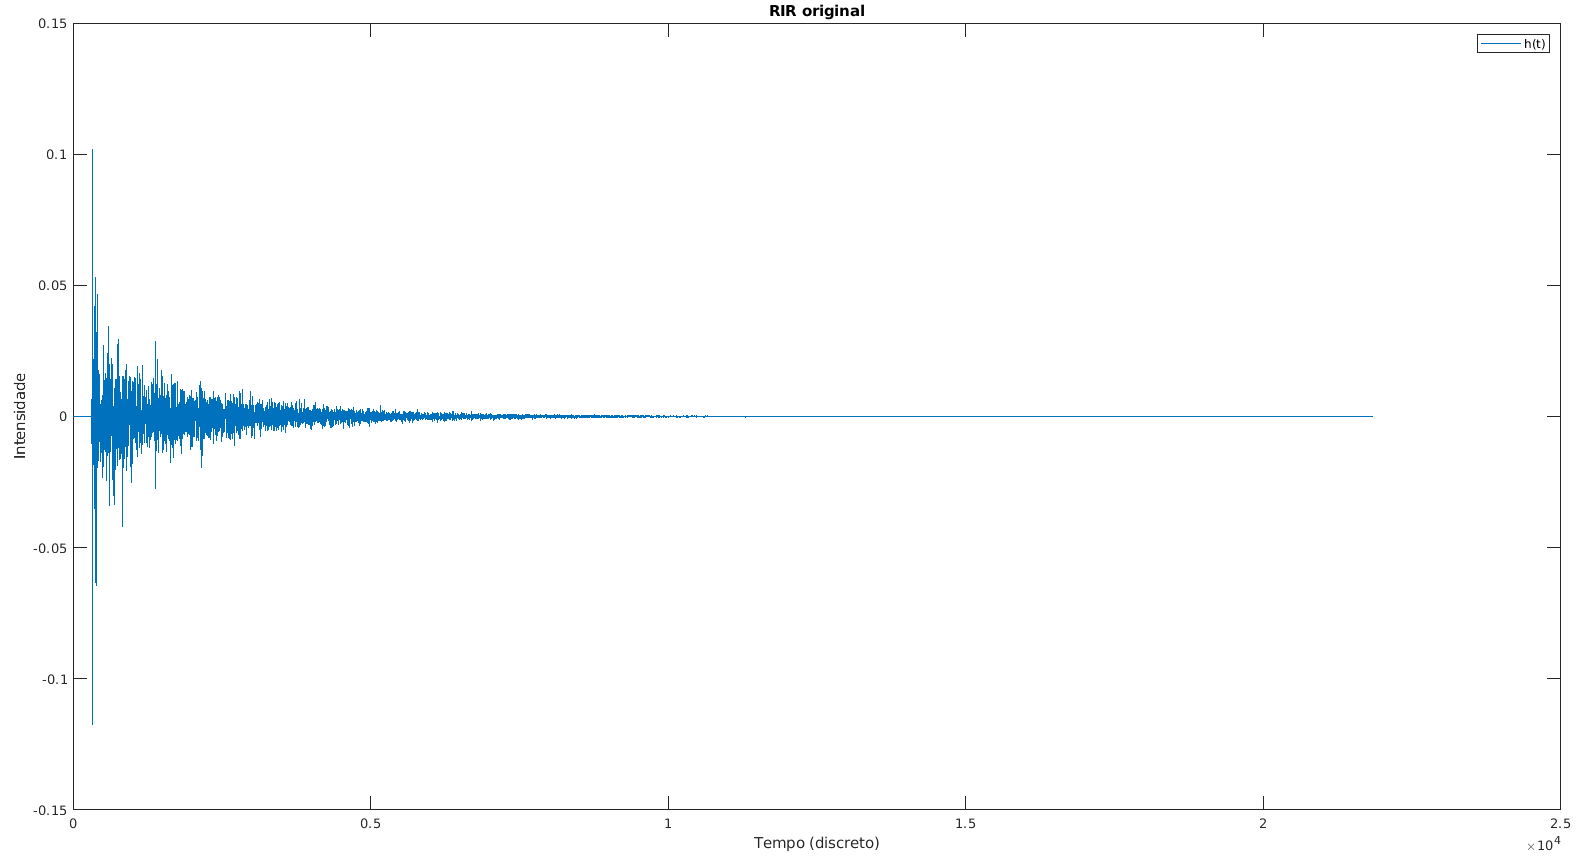
\includegraphics[scale=0.115]{rir-og-d1.png}
            \end{subfigure}
            \begin{subfigure}{\textwidth}
                \centering
                \notextattachfile{\scriptsize RIR Simulada}
                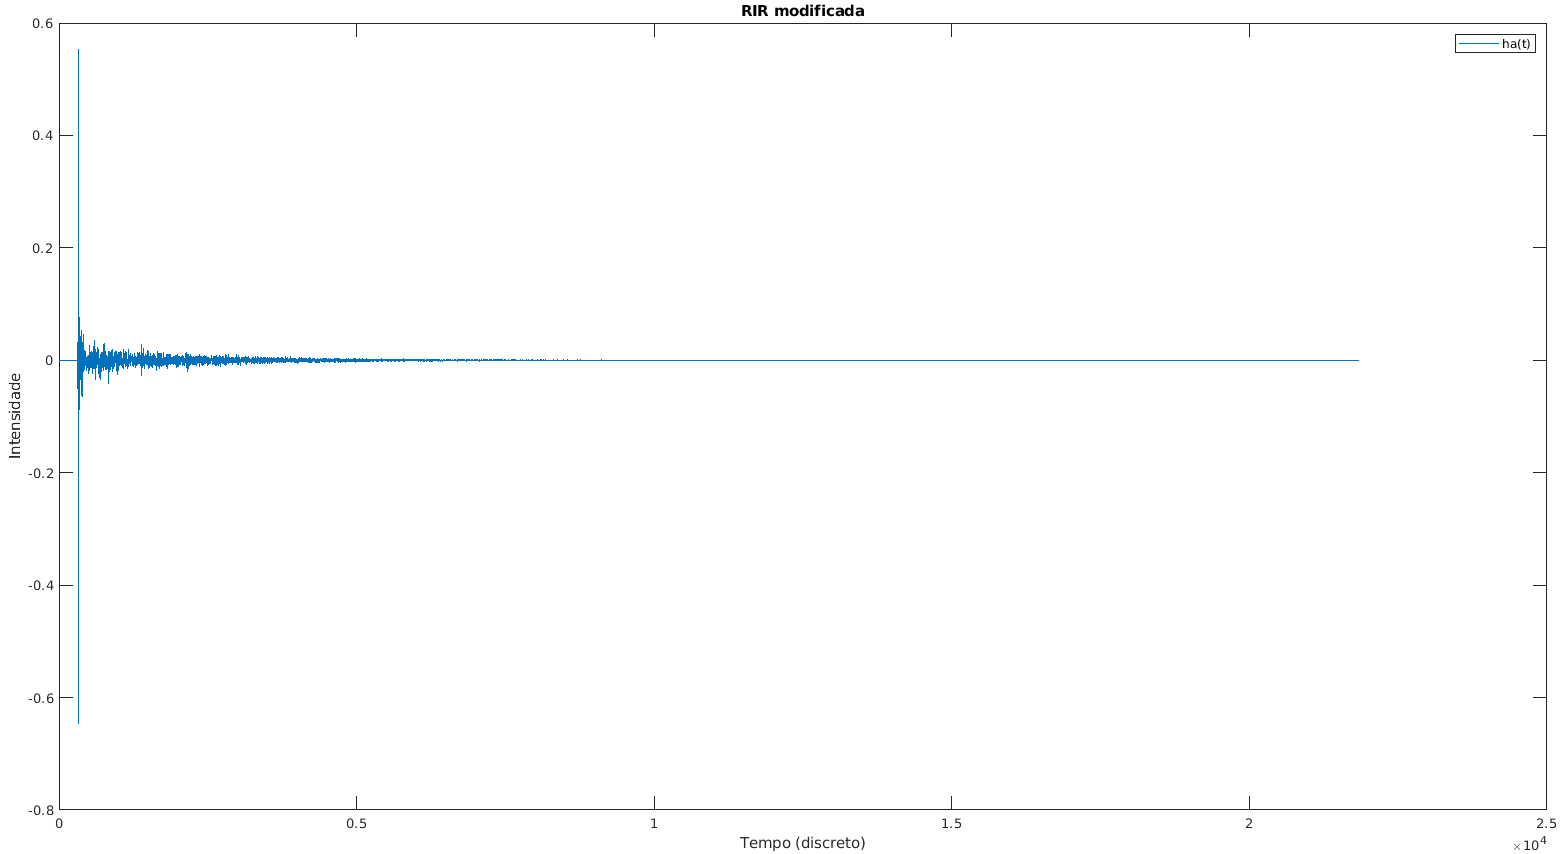
\includegraphics[scale=0.115]{rir-aug-d1.png}
            \end{subfigure}
        \end{figure}
    \end{columns}
        
\end{frame}

\begin{frame}{Exemplo D1}
    \begin{columns}
        \column{0.5\textwidth}
        \begin{figure}
            \begin{subfigure}{\textwidth}
                \centering
                \textattachfile{audios/voice-og-d1.wav}{\scriptsize amostra de voz original}
                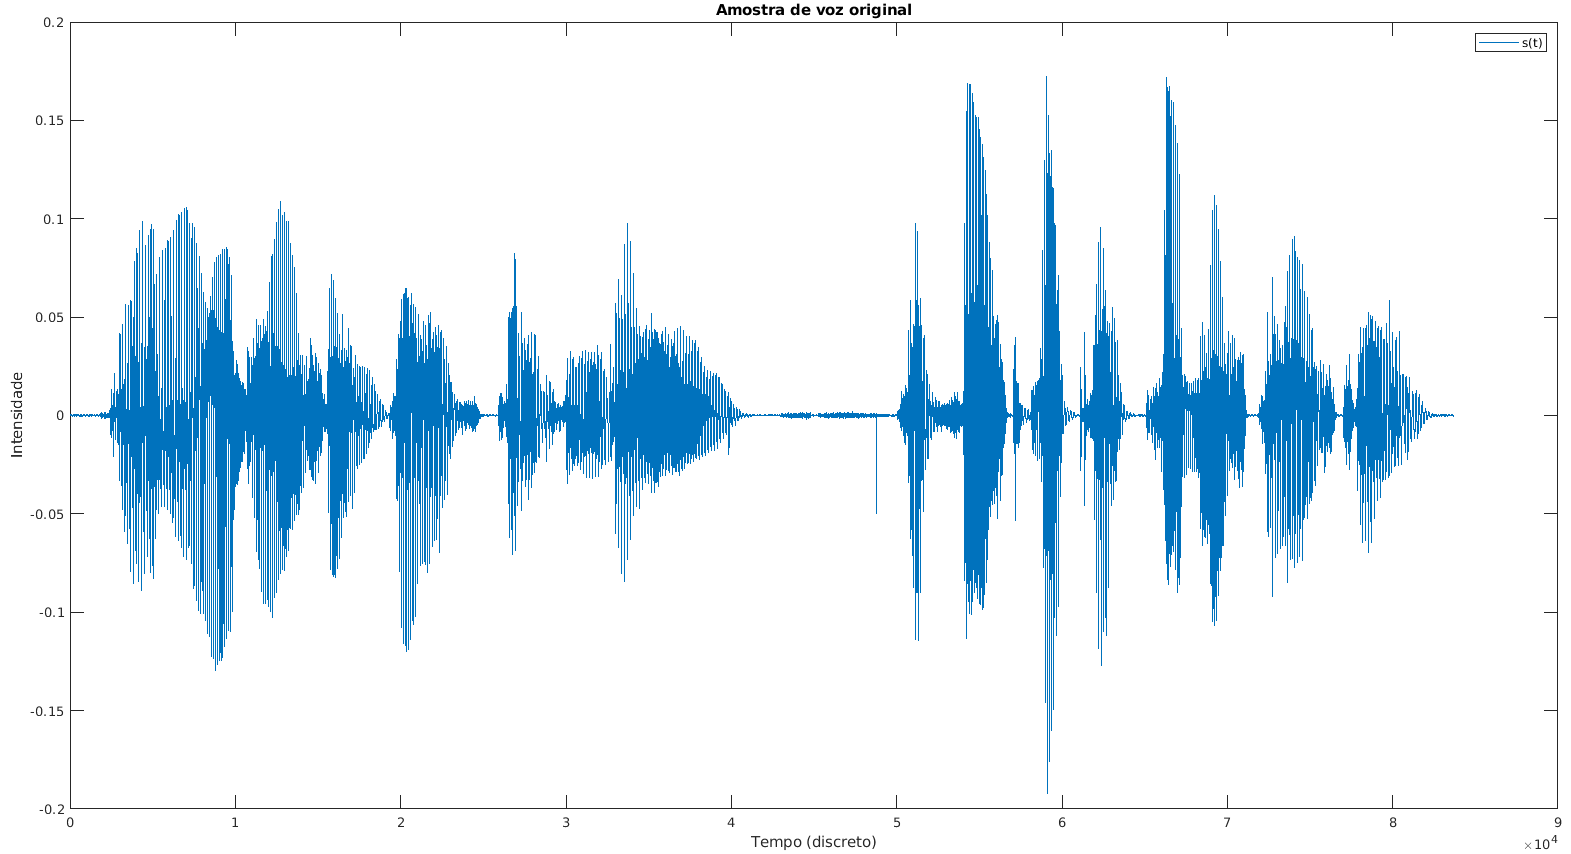
\includegraphics[scale=0.105]{voice-og-d1.png}
            \end{subfigure}
        \end{figure}

        \column{0.5\textwidth}
        \begin{figure}
            \begin{subfigure}{\textwidth}
                \centering
                \textattachfile{audios/voice-aug-riro-d1.wav}{\footnotesize amostra de voz reverberada - RIRO}
                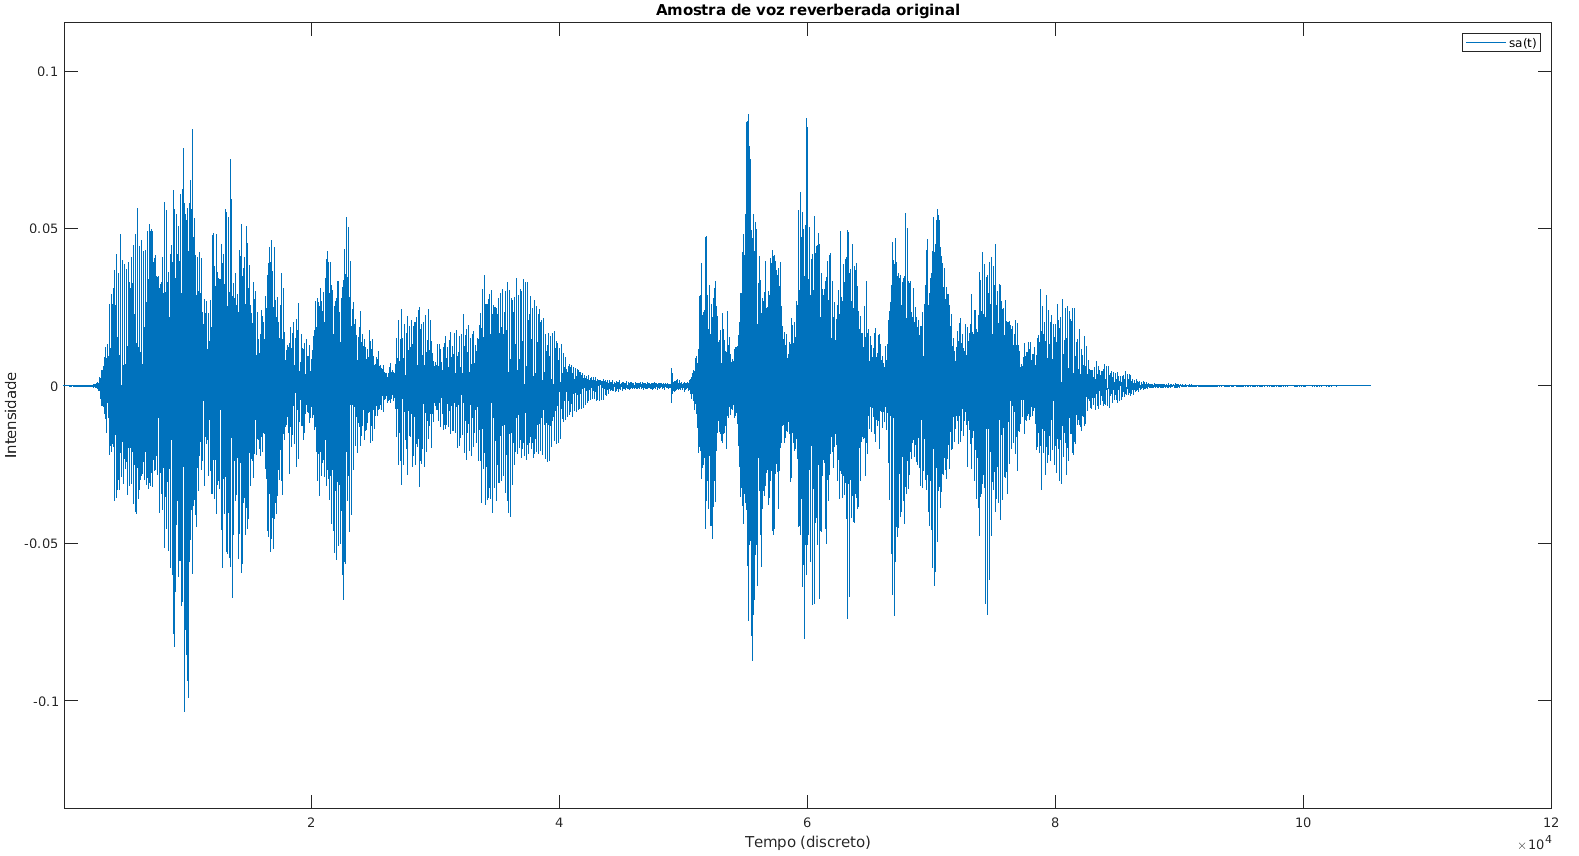
\includegraphics[scale=0.105]{voice-aug-riro-d1.png}
            \end{subfigure}
            \begin{subfigure}{\textwidth}
                \centering
                \textattachfile{audios/voice-aug-d1.wav}{\footnotesize amostra de voz reverberada - RIRSM}
                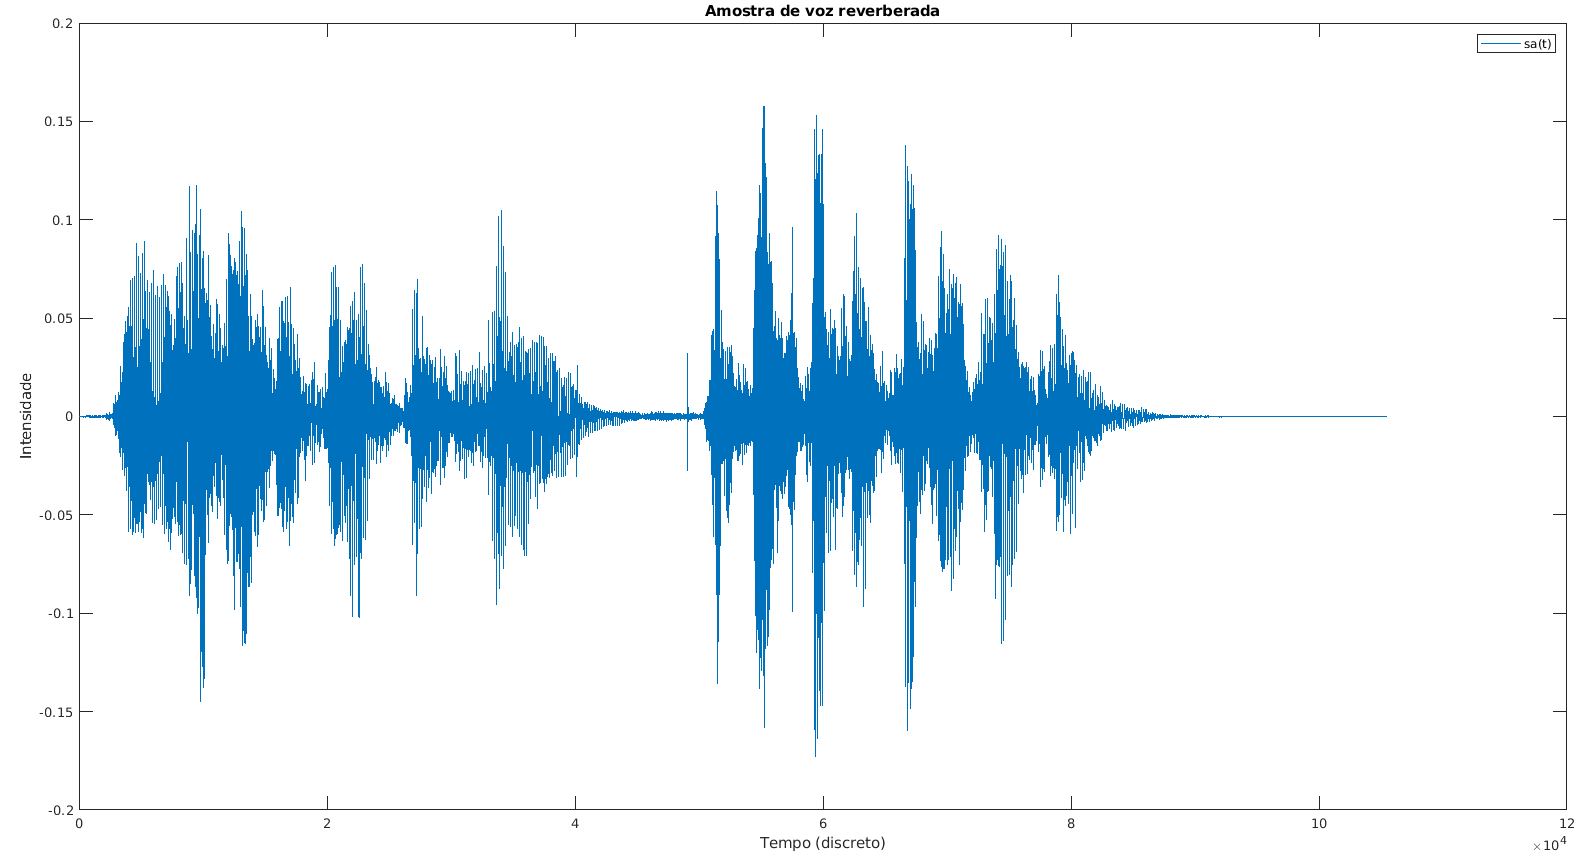
\includegraphics[scale=0.105]{voice-aug-d1.png}
            \end{subfigure}
        \end{figure}
    \end{columns}
\end{frame}

\begin{frame}{Exemplo D2}
    \begin{columns}
        \column{.6\textwidth}
        \begin{figure}
            \begin{subfigure}{\textwidth}
                \centering
                \notextattachfile{\scriptsize RIR Original}
                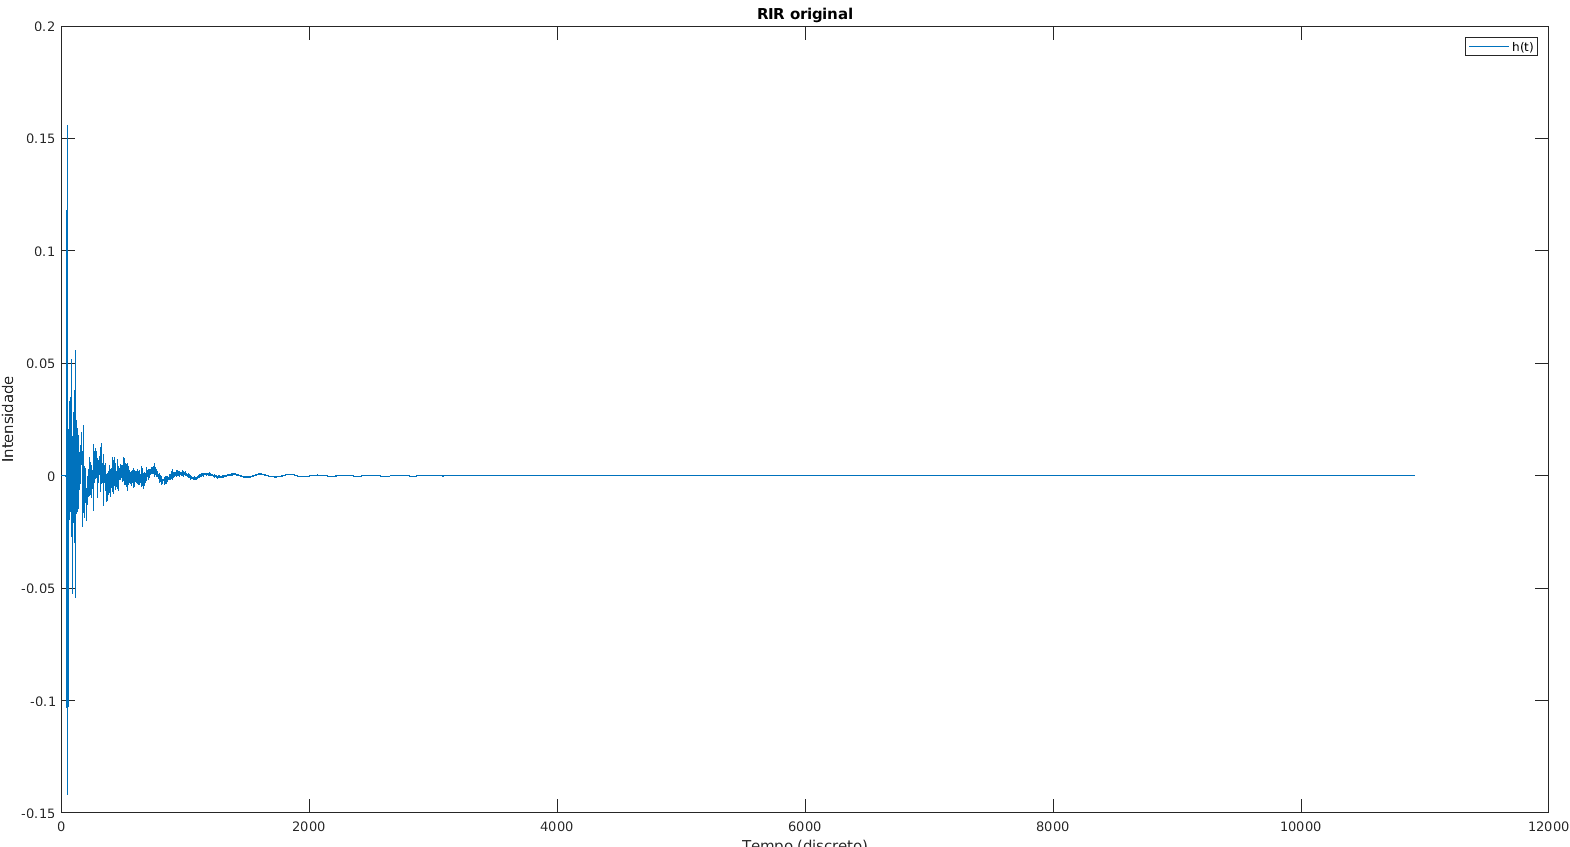
\includegraphics[scale=0.115]{rir-og-d2.png}
            \end{subfigure}
            \begin{subfigure}{\textwidth}
                \centering
                \notextattachfile{\scriptsize RIR Simulada}
                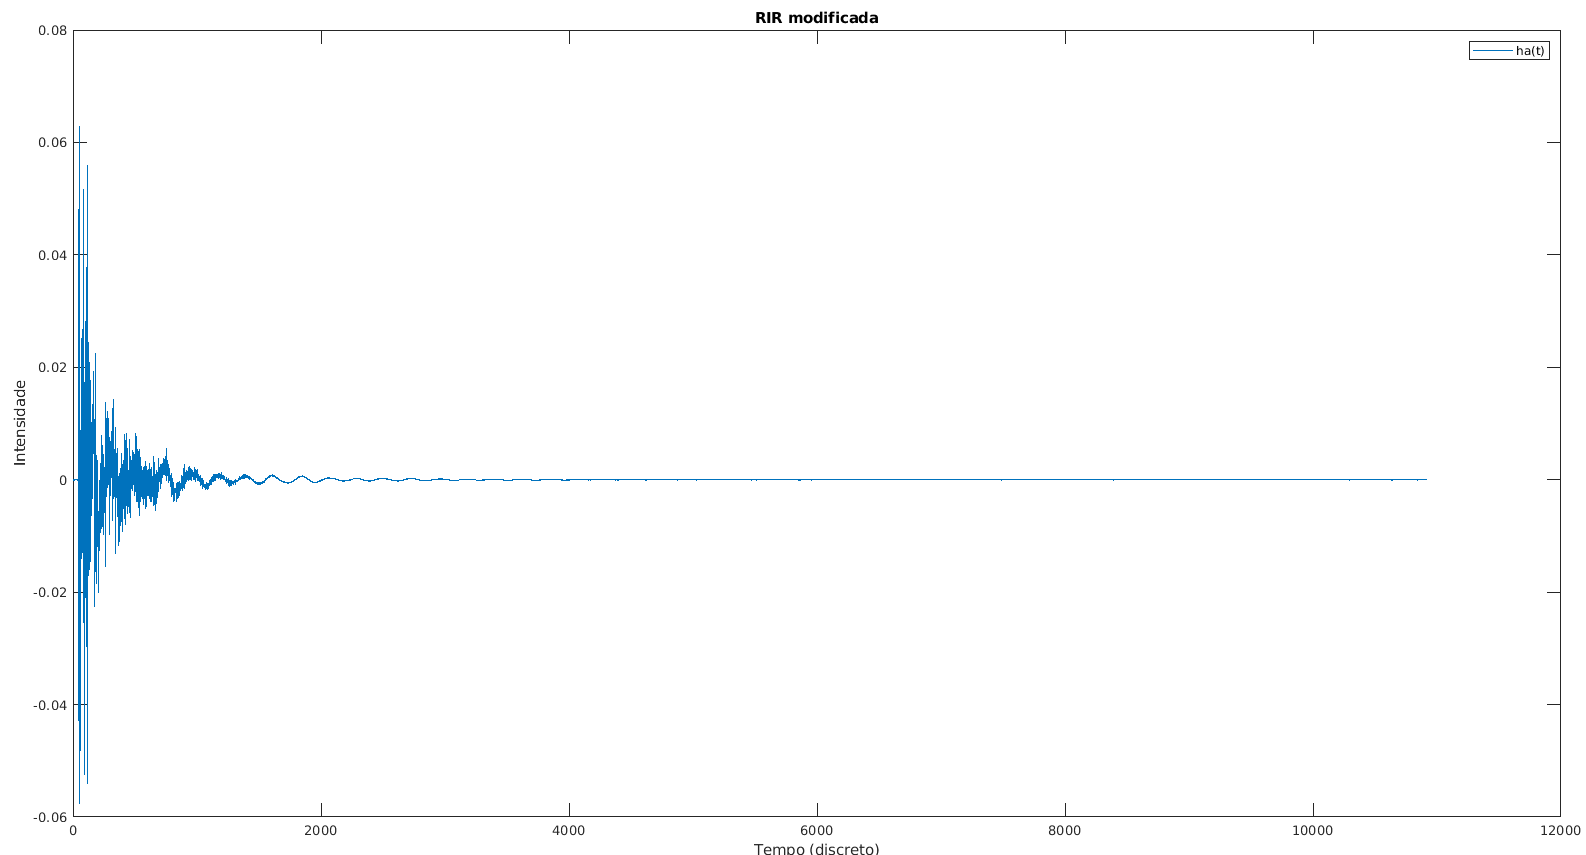
\includegraphics[scale=0.115]{rir-aug-d2.png}
            \end{subfigure}
        \end{figure}
    \end{columns}
        
\end{frame}

\begin{frame}{Exemplo D2}
    \begin{columns}
        \column{0.5\textwidth}
        \begin{figure}
            \begin{subfigure}{\textwidth}
                \centering
                \textattachfile{audios/voice-og-d2.wav}{\scriptsize amostra de voz original}
                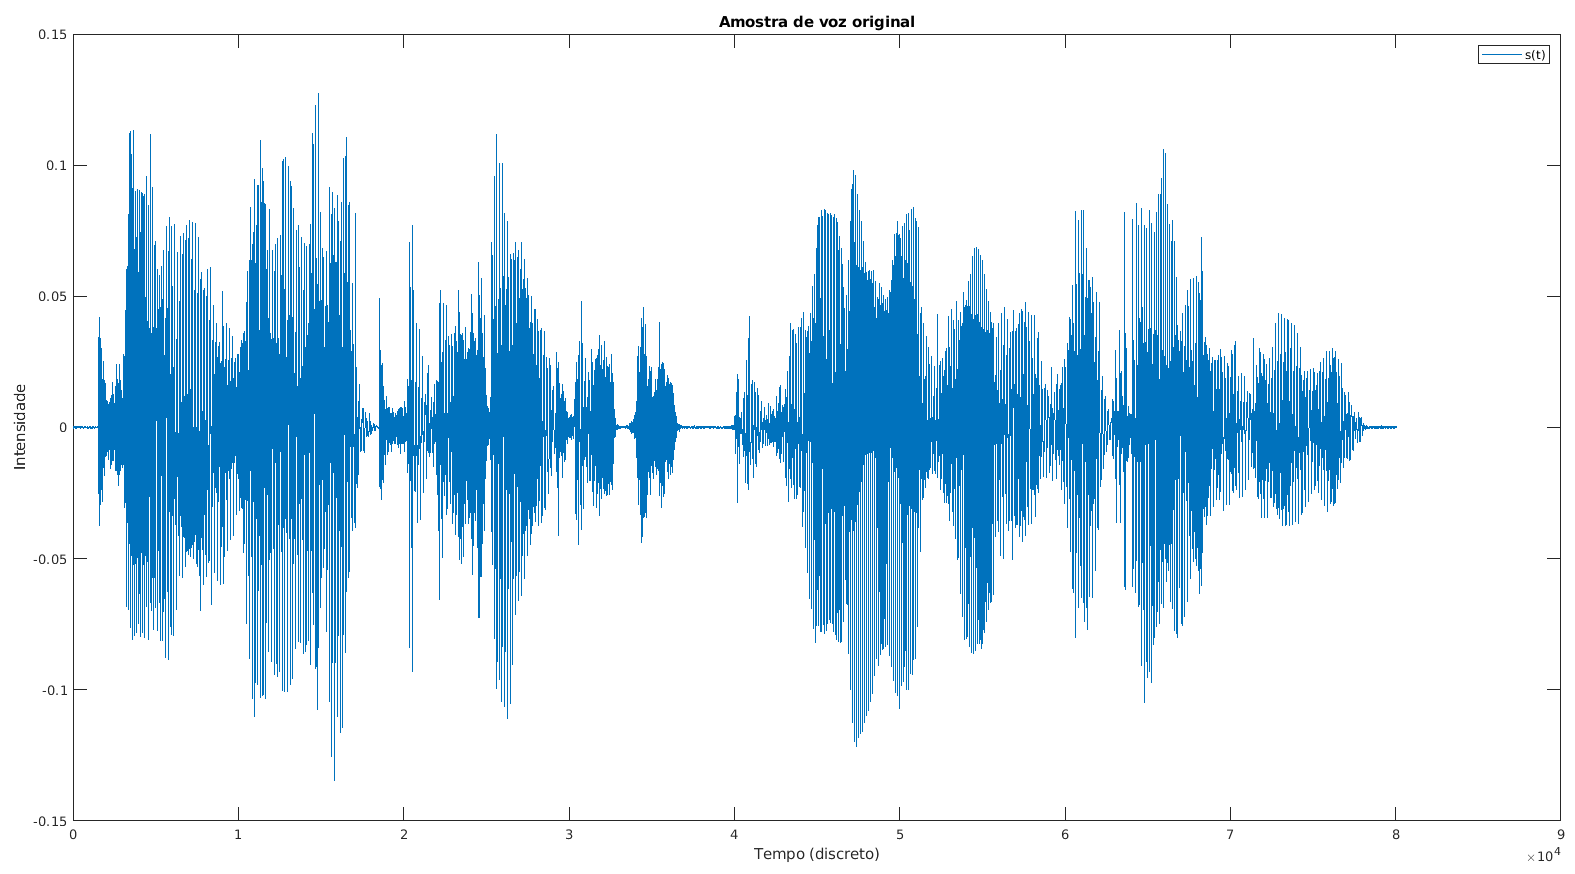
\includegraphics[scale=0.105]{voice-og-d2.png}
            \end{subfigure}
        \end{figure}

        \column{0.5\textwidth}
        \begin{figure}
            \begin{subfigure}{\textwidth}
                \centering
                \textattachfile{audios/voice-aug-riro-d2.wav}{\footnotesize amostra de voz reverberada - RIRO}
                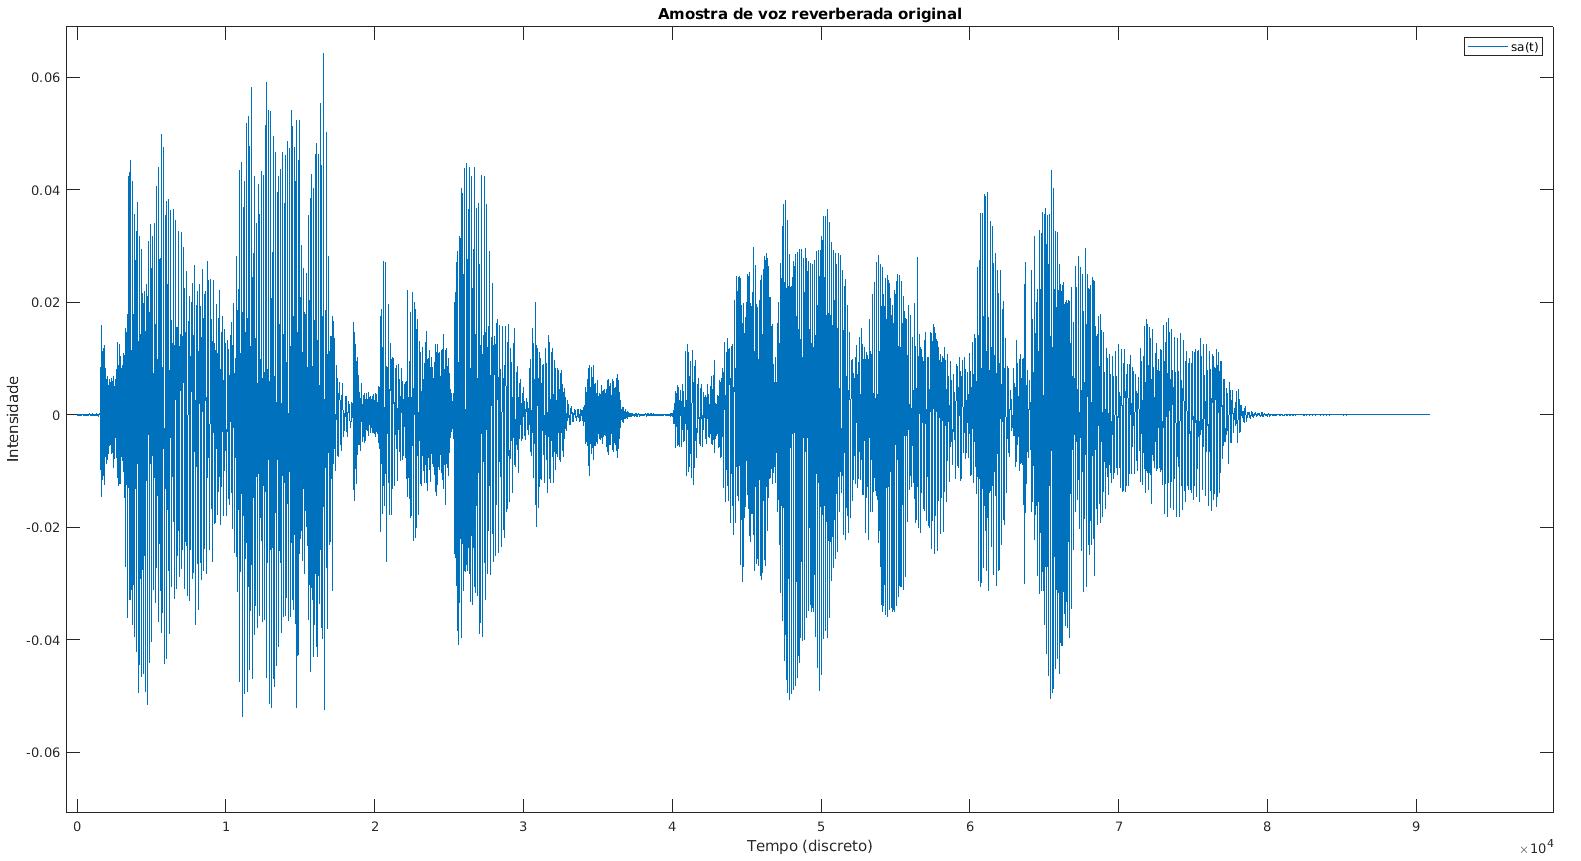
\includegraphics[scale=0.105]{voice-aug-riro-d2.png}
            \end{subfigure}
            \begin{subfigure}{\textwidth}
                \centering
                \textattachfile{audios/voice-aug-d2.wav}{\footnotesize amostra de voz reverberada - RIRSM}
                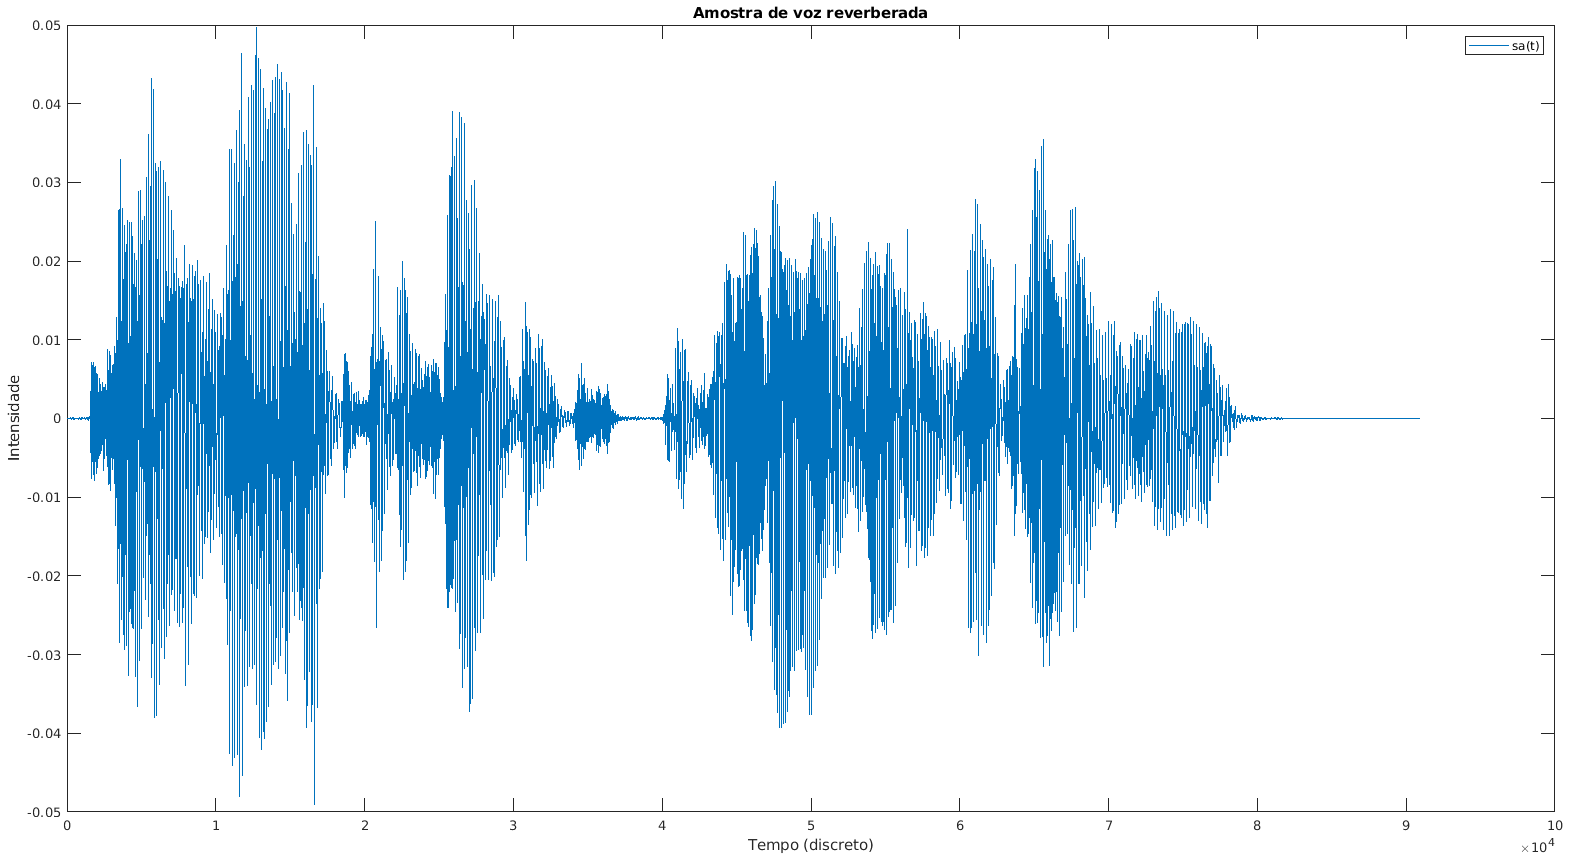
\includegraphics[scale=0.105]{voice-aug-d2.png}
            \end{subfigure}
        \end{figure}
    \end{columns}
\end{frame}

%% ---------------------------------------------------------------------------
% RESULTADOS - T60

\begin{frame}{Resultados - T60}
    \begin{table} [H]
        \centering
        \begin{tabular}{c|c|c|c}
    
            \textbf{Exemplo} & 
            \textbf{Sala RIR} & 
            \textbf{Distância (m)} &
            \textbf{Amostra de Voz} \\
            \hline 
    
            T1 & lecture & 7.1 & M2-T1 \\
            T2 & booth & 1 & H1-T2 \\
            T3 & office & 2 & H2-T2 \\
    
        \end{tabular}
        \bigbreak
        \bigbreak
        \begin{tabular}{c|c|c|c|c}
    
            \textbf{Exemplo} & 
            \textbf{$T60_{org}$ (s)} & 
            \textbf{$T60_{alvo}$ (s)} &
            \textbf{$T60_{res}$ (s)} & 
            \textbf{$\rho_{T60}$ (\%)} \\
            \hline 
    
            T1 & 1,38 & 1,15 & 1,01 & 12.1 \\
            T2 & 1,01 & 1,88 & 1,89 & 0,5 \\
            T3 & 0,75 & 0,61 & 0,60 & 1,6 \\
    
        \end{tabular}
        \vspace{0.5cm}

        $\rho_{T60} = |T60_{res} - T60_{alvo}|/T60_{alvo}$
    \end{table}
\end{frame}

\begin{frame}{Resultados - T60}
    \textbf{Experimento empírico}: sensação subjetiva de “eco”, ordenado de mais para menos ecoante.
    \vspace{1cm}

    \begin{table} [H]
        \centering
        \begin{tabular}{c|c|c|c|c}
    
            \textbf{Exemplo} & 
            \textbf{$T60_{org}$ (s)} & 
            \textbf{$T60_{res}$ (s)} & 
            \textbf{Comparação} &
            \textbf{Ordem} \\
            \hline 
    
            T1 & 1,38 & 1,01 & original & 2 \\
            T2 & 1,01 & 1,89 & simulado & 1 \\
            T3 & 0,75 & 0,60 & original & 3 \\
    
        \end{tabular}
    \end{table}
\end{frame}

\begin{frame}{Exemplo T1}
    \begin{columns}
        \column{.6\textwidth}
        \begin{figure}
            \begin{subfigure}{\textwidth}
                \centering
                \notextattachfile{\scriptsize RIR Original}
                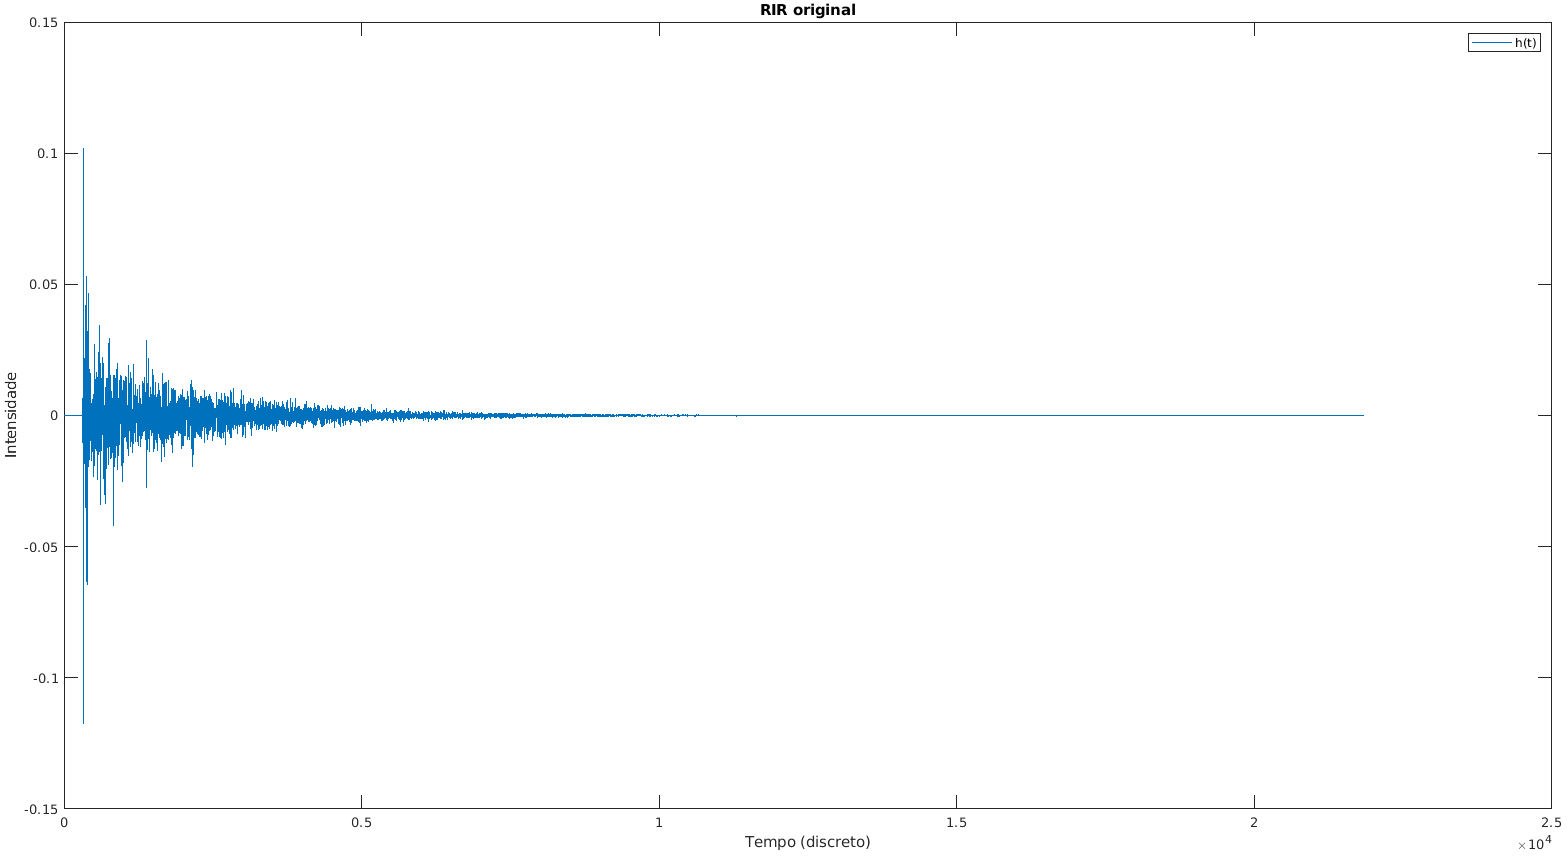
\includegraphics[scale=0.115]{rir-og-t1.png}
            \end{subfigure}
            \begin{subfigure}{\textwidth}
                \centering
                \notextattachfile{\scriptsize RIR Simulada}
                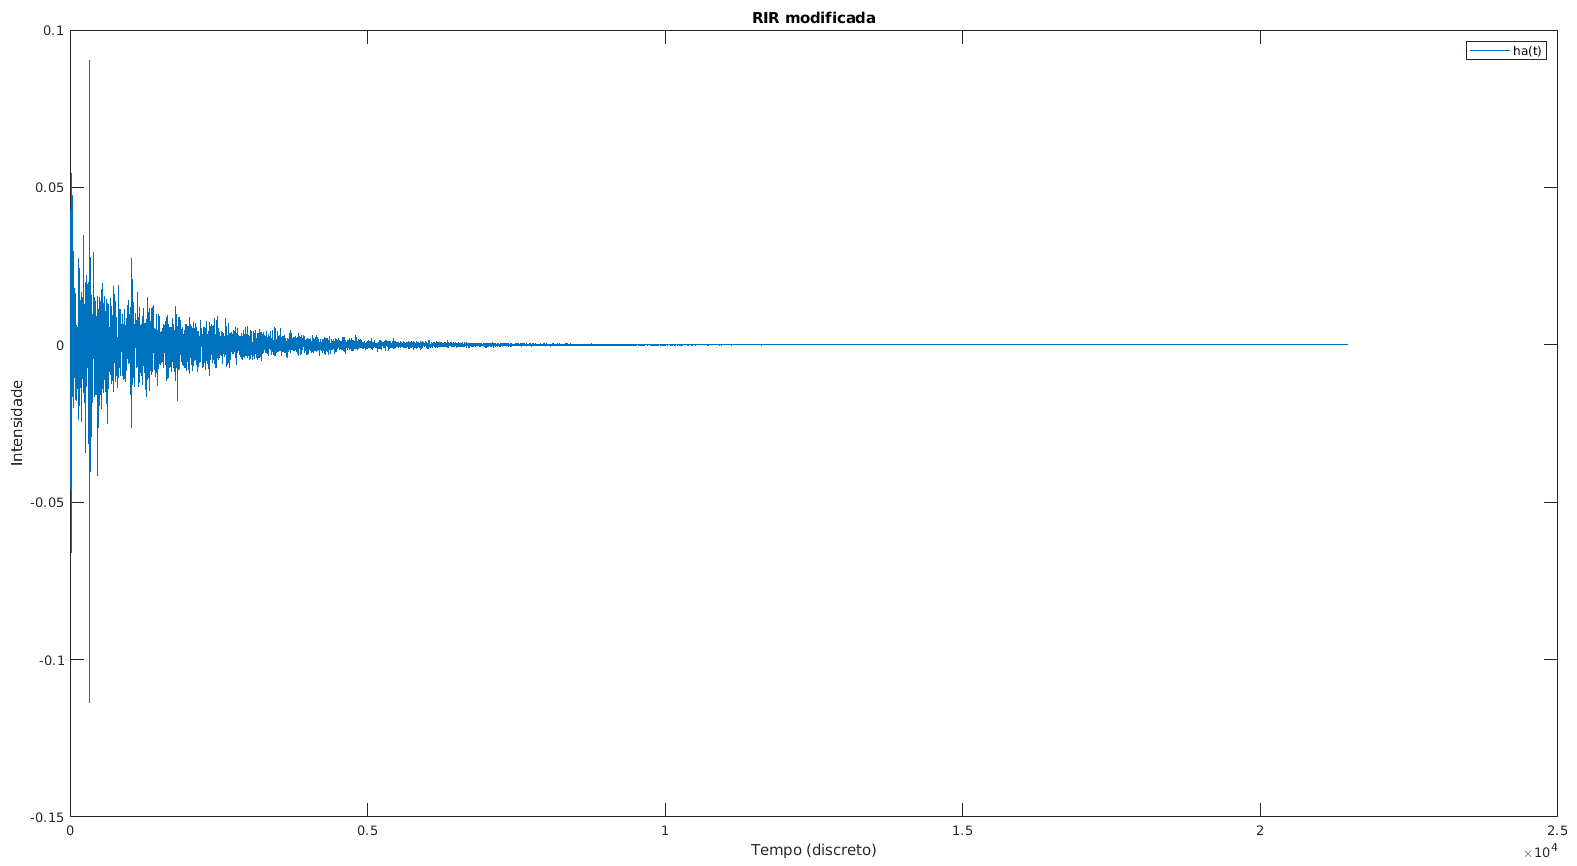
\includegraphics[scale=0.115]{rir-aug-t1.png}
            \end{subfigure}
        \end{figure}
    \end{columns}
        
\end{frame}

\begin{frame}{Exemplo T1}
    \begin{columns}
        \column{0.5\textwidth}
        \begin{figure}
            \begin{subfigure}{\textwidth}
                \centering
                \textattachfile{audios/voice-og-t1.wav}{\scriptsize amostra de voz original}
                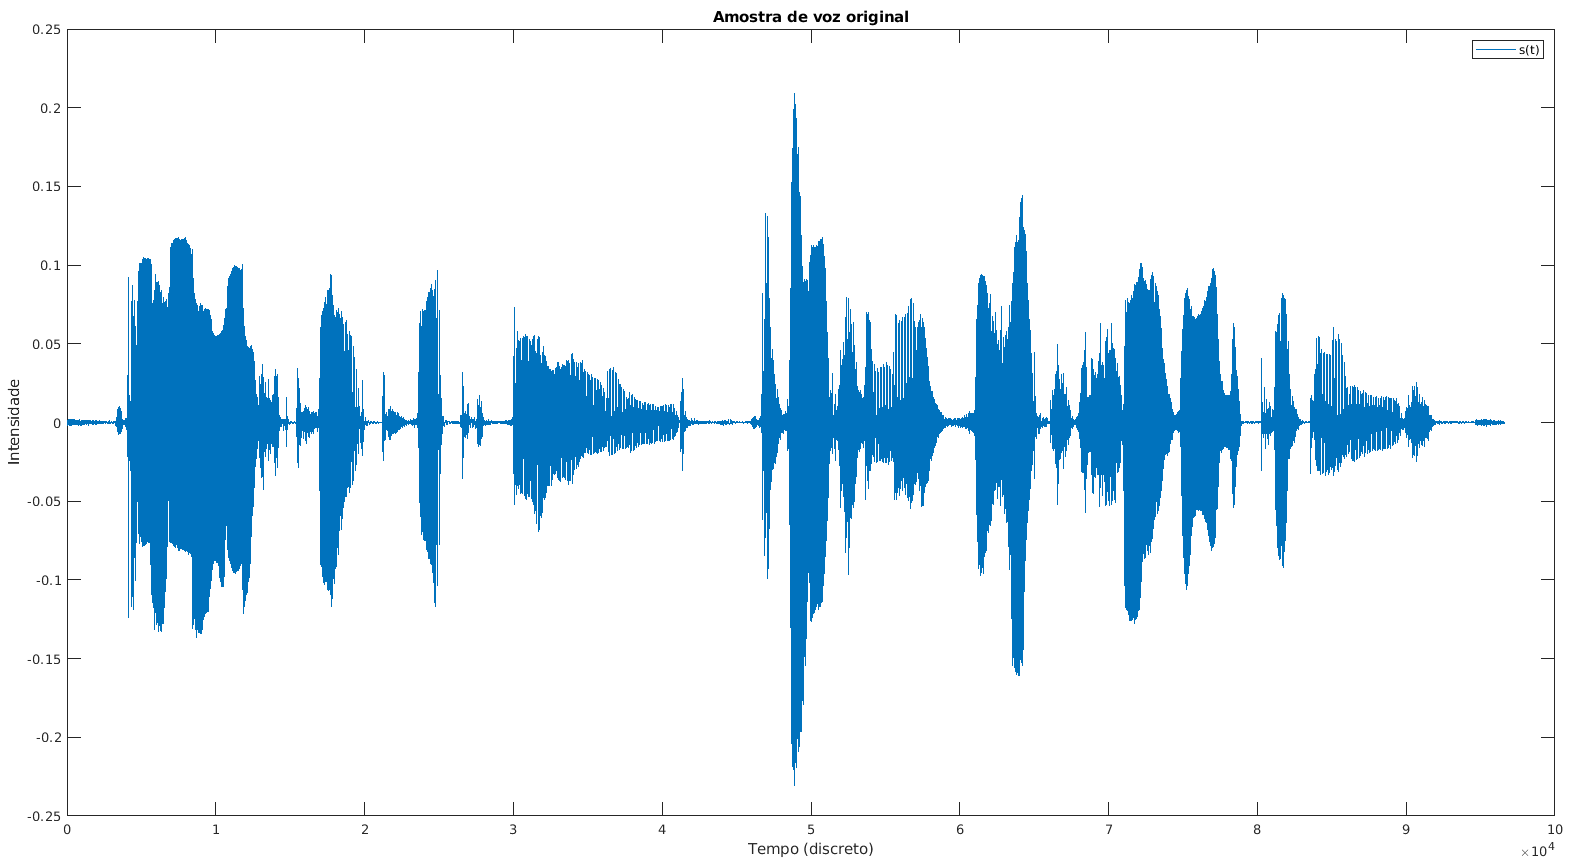
\includegraphics[scale=0.105]{voice-og-t1.png}
            \end{subfigure}
        \end{figure}

        \column{0.5\textwidth}
        \begin{figure}
            \begin{subfigure}{\textwidth}
                \centering
                \textattachfile{audios/voice-aug-riro-t1.wav}{\footnotesize amostra de voz reverberada - RIRO}
                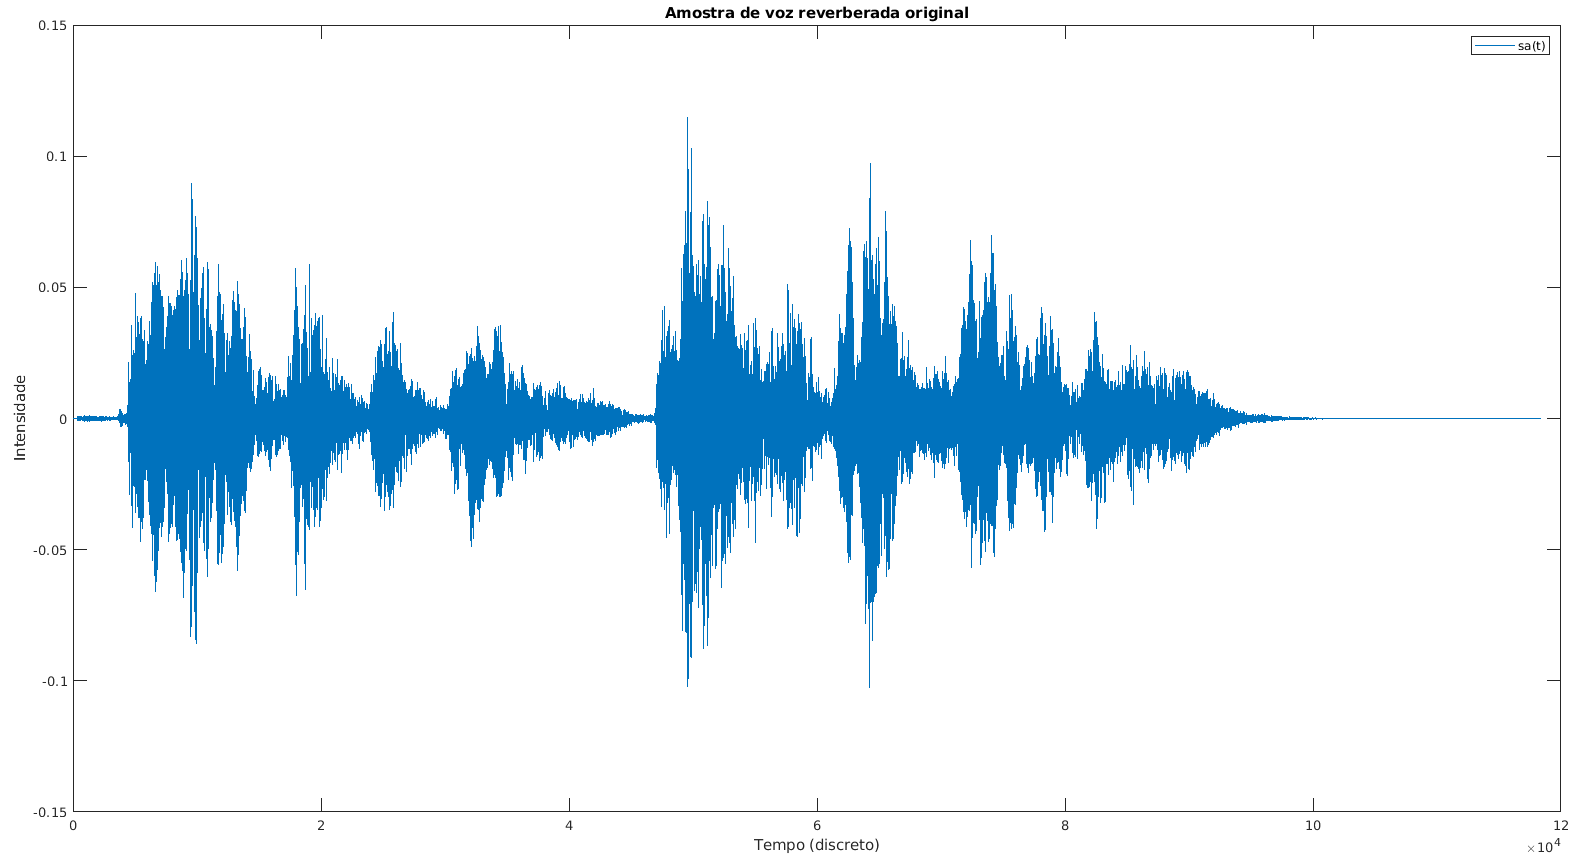
\includegraphics[scale=0.105]{voice-aug-riro-t1.png}
            \end{subfigure}
            \begin{subfigure}{\textwidth}
                \centering
                \textattachfile{audios/voice-aug-t1.wav}{\footnotesize amostra de voz reverberada - RIRSM}
                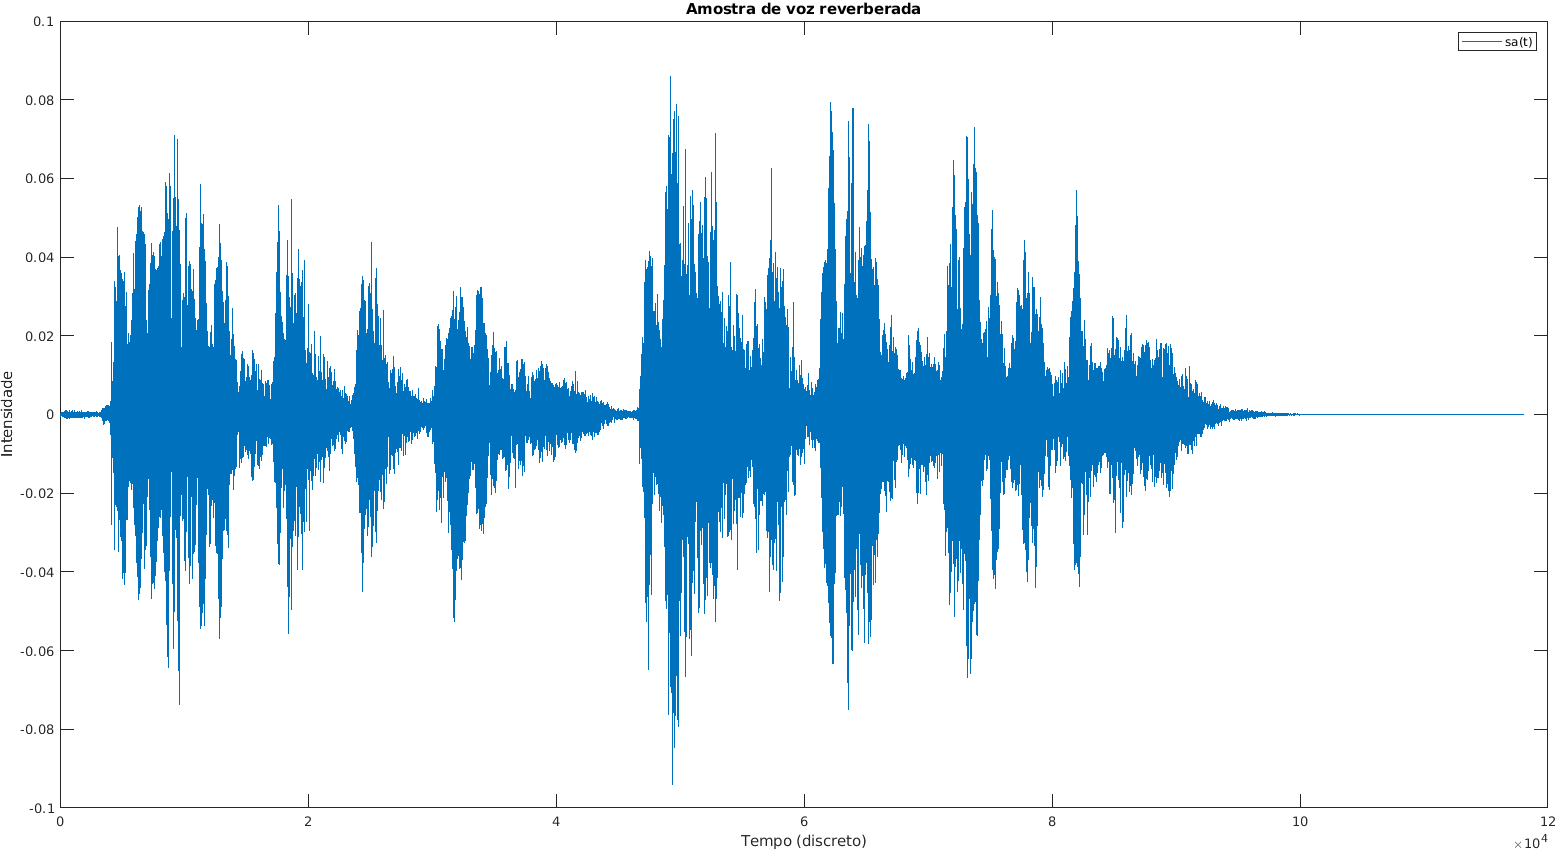
\includegraphics[scale=0.105]{voice-aug-t1.png}
            \end{subfigure}
        \end{figure}
    \end{columns}
\end{frame}

\begin{frame}{Exemplo T2}
    \begin{columns}
        \column{.6\textwidth}
        \begin{figure}
            \begin{subfigure}{\textwidth}
                \centering
                \notextattachfile{\scriptsize RIR Original}
                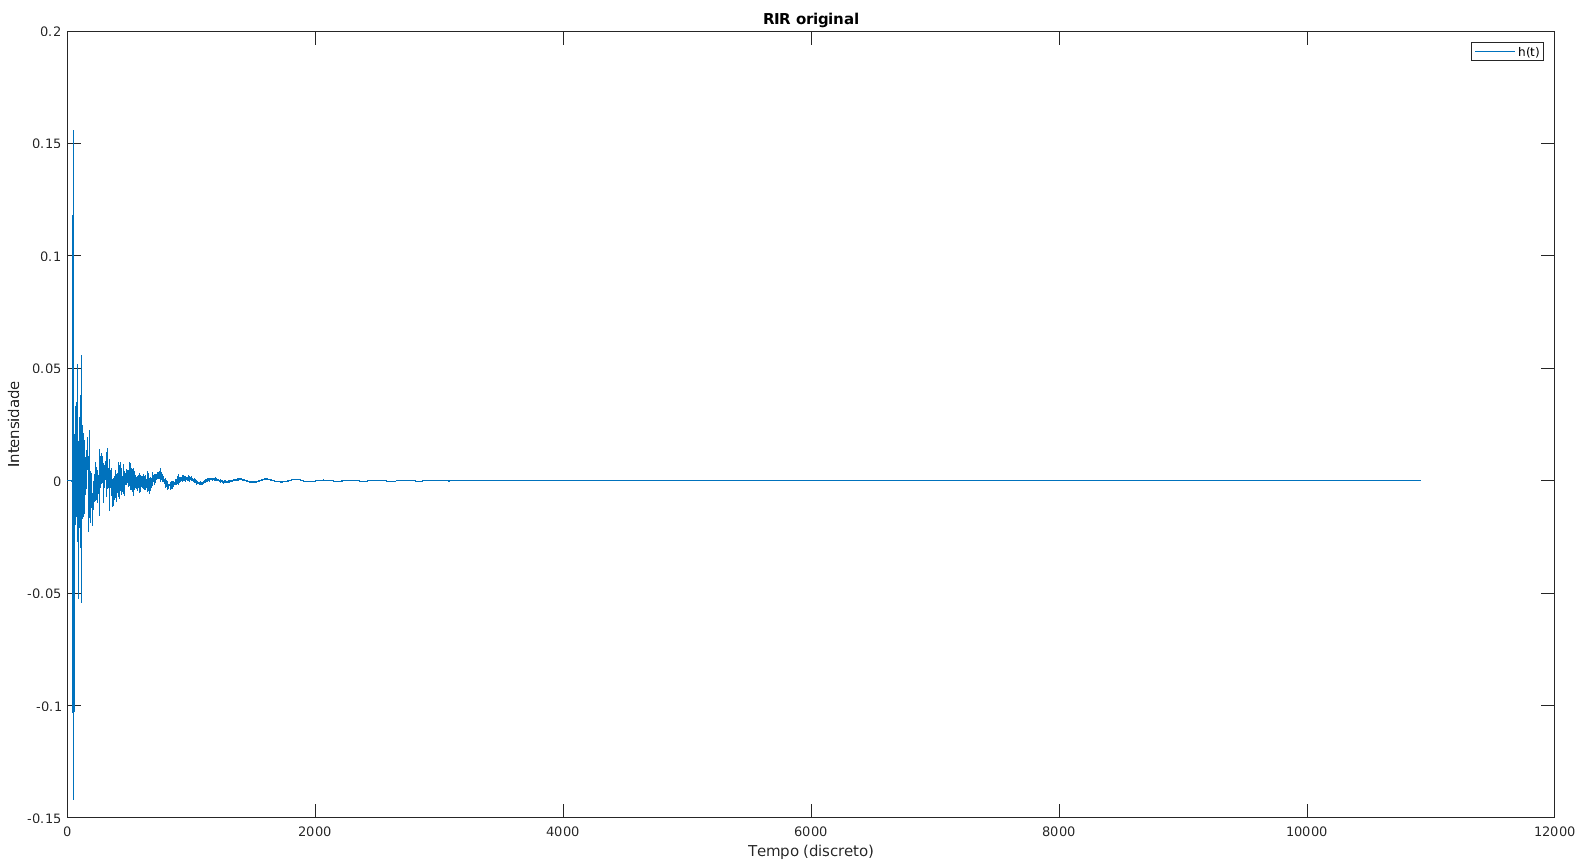
\includegraphics[scale=0.115]{rir-og-t2.png}
            \end{subfigure}
            \begin{subfigure}{\textwidth}
                \centering
                \notextattachfile{\scriptsize RIR Simulada}
                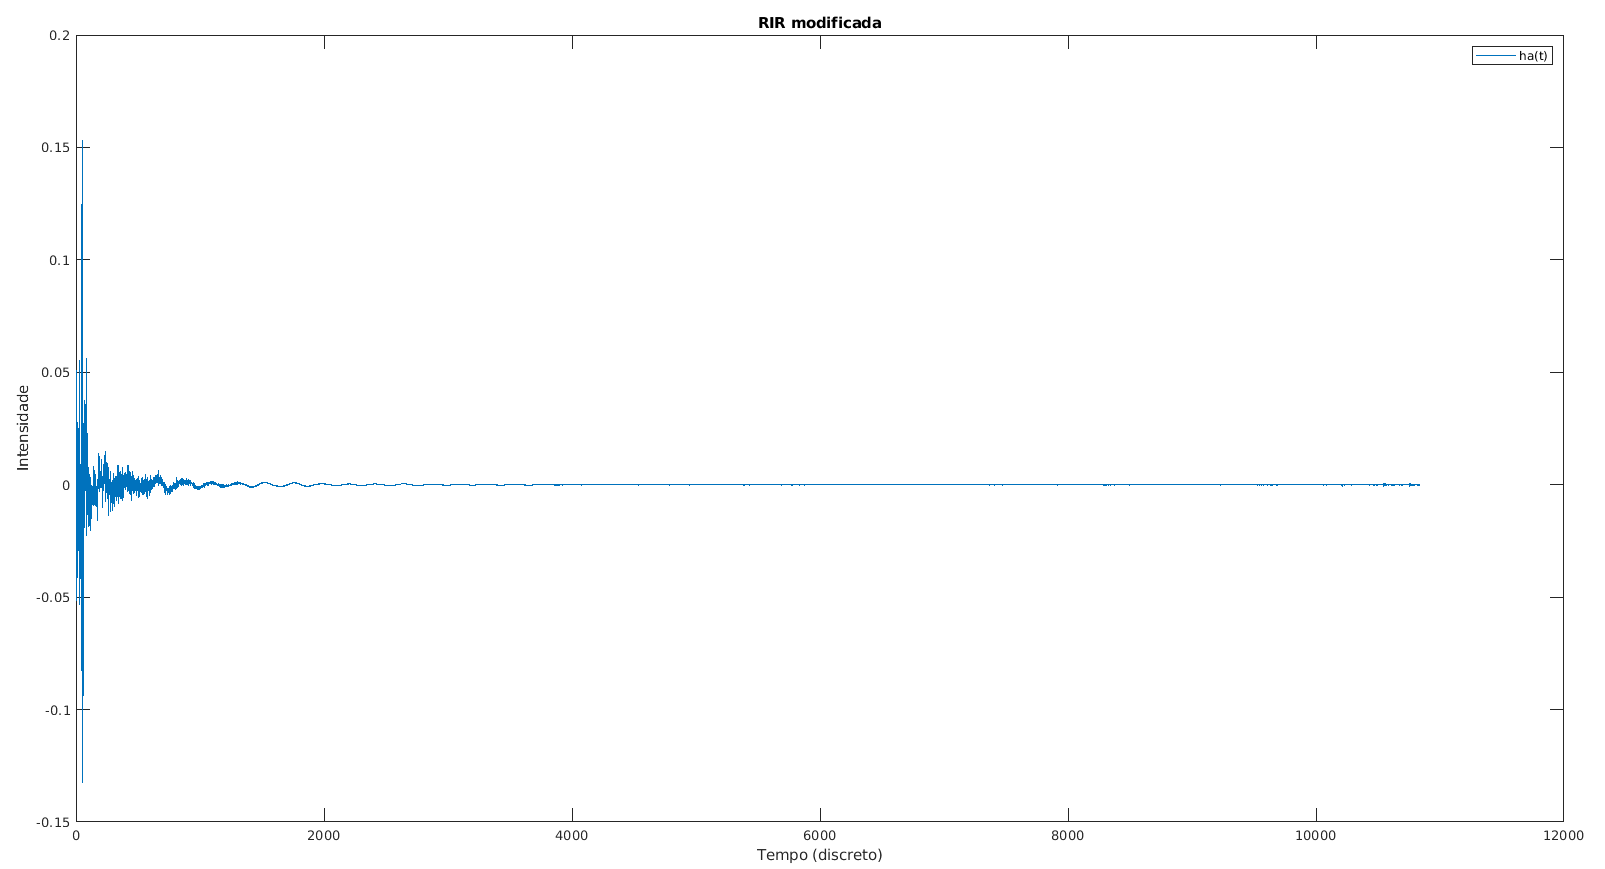
\includegraphics[scale=0.115]{rir-aug-t2.png}
            \end{subfigure}
        \end{figure}
    \end{columns}
        
\end{frame}

\begin{frame}{Exemplo T2}
    \begin{columns}
        \column{0.5\textwidth}
        \begin{figure}
            \begin{subfigure}{\textwidth}
                \centering
                \textattachfile{audios/voice-og-t2.wav}{\scriptsize amostra de voz original}
                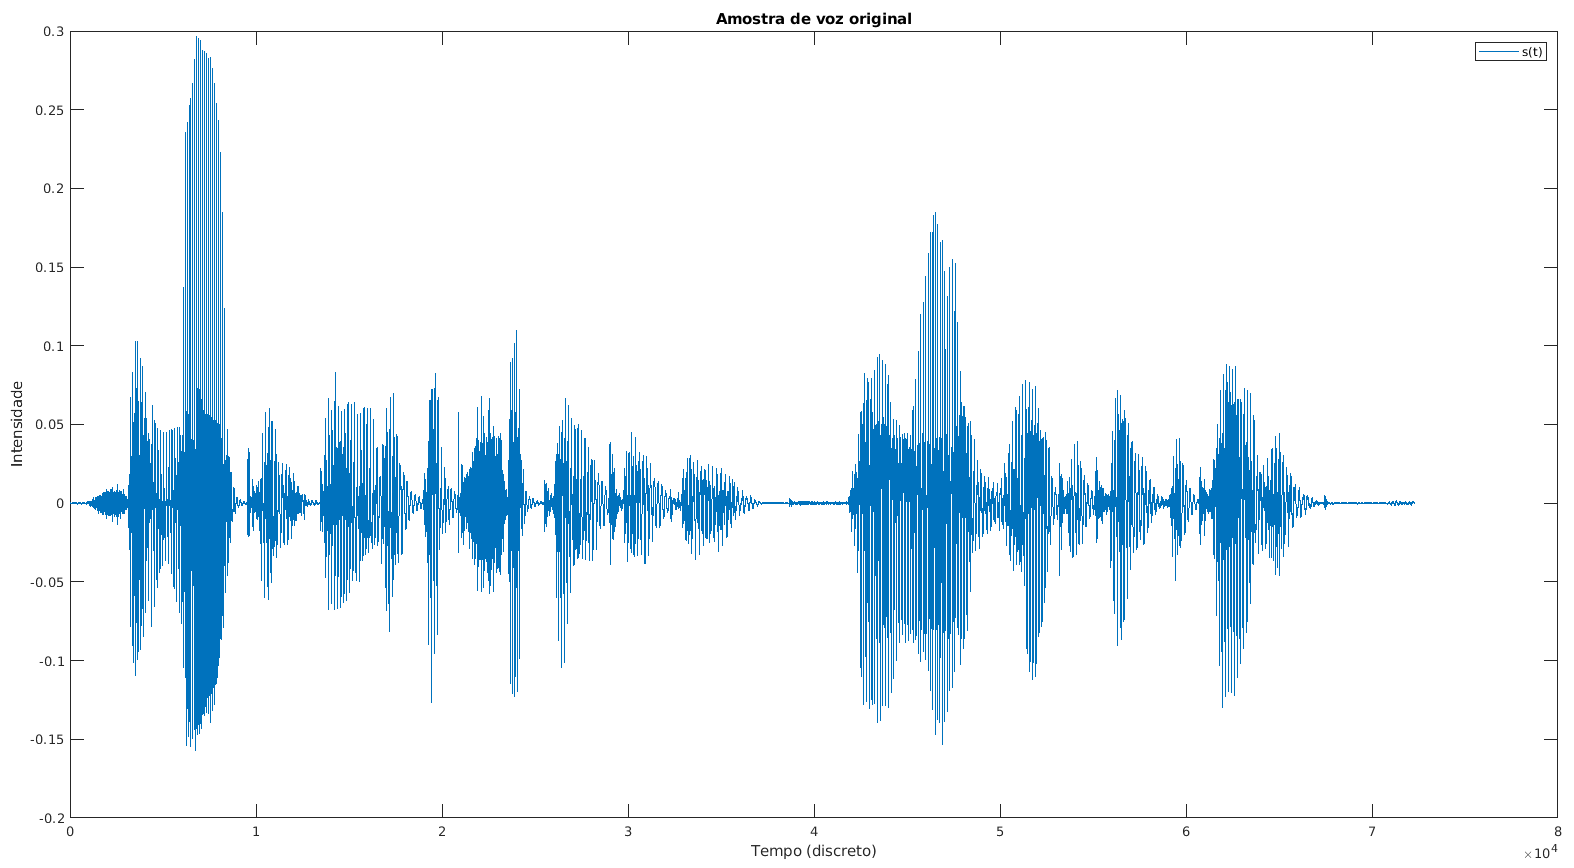
\includegraphics[scale=0.105]{voice-og-t2.png}
            \end{subfigure}
        \end{figure}

        \column{0.5\textwidth}
        \begin{figure}
            \begin{subfigure}{\textwidth}
                \centering
                \textattachfile{audios/voice-aug-riro-t2.wav}{\footnotesize amostra de voz reverberada - RIRO}
                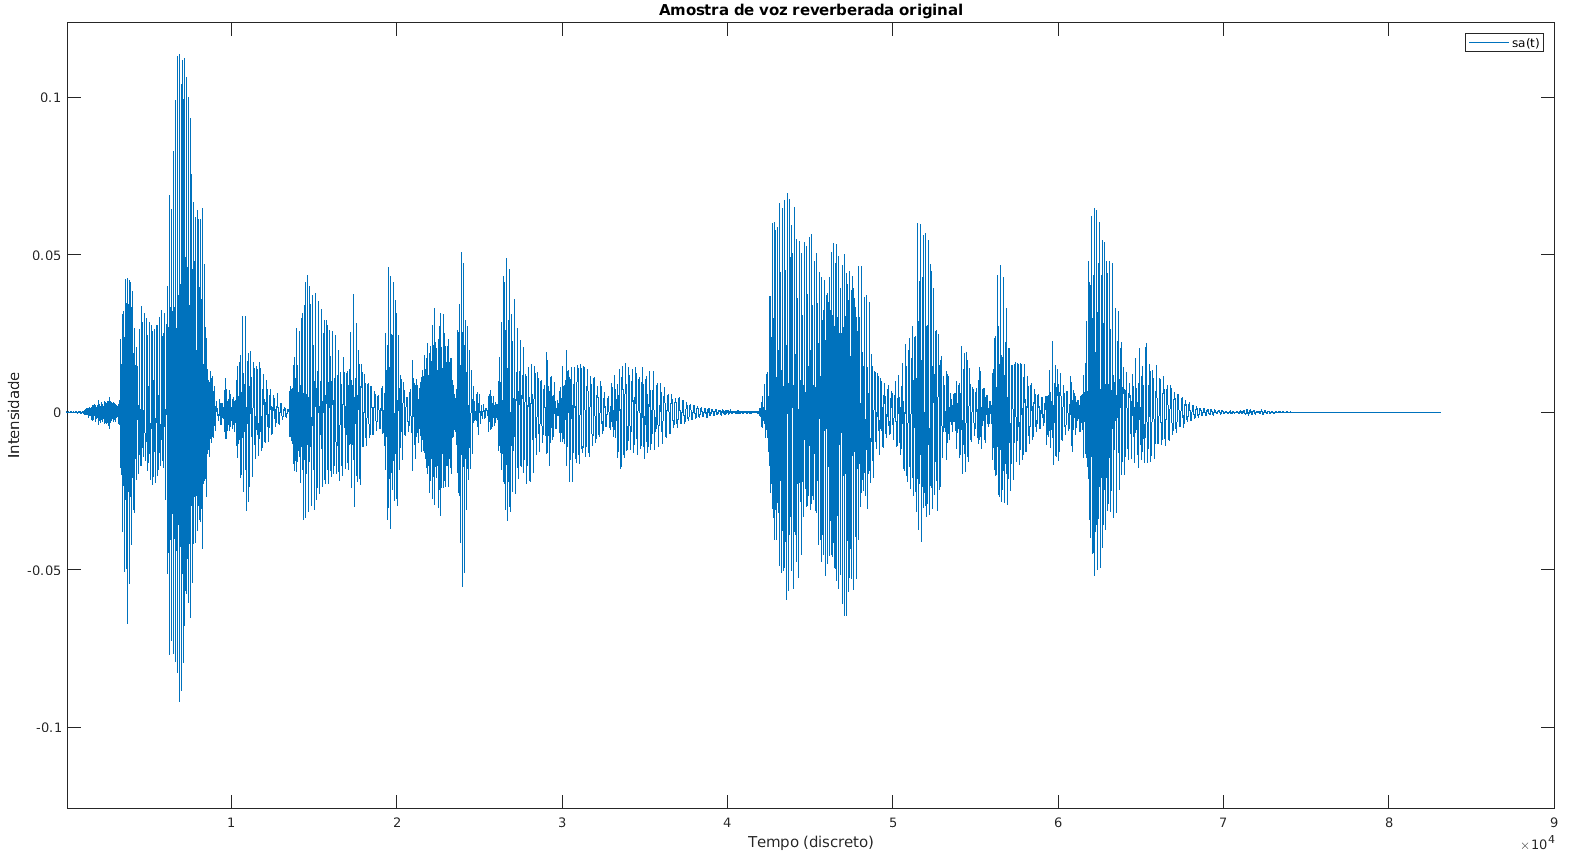
\includegraphics[scale=0.105]{voice-aug-riro-t2.png}
            \end{subfigure}
            \begin{subfigure}{\textwidth}
                \centering
                \textattachfile{audios/voice-aug-t2.wav}{\footnotesize amostra de voz reverberada - RIRSM}
                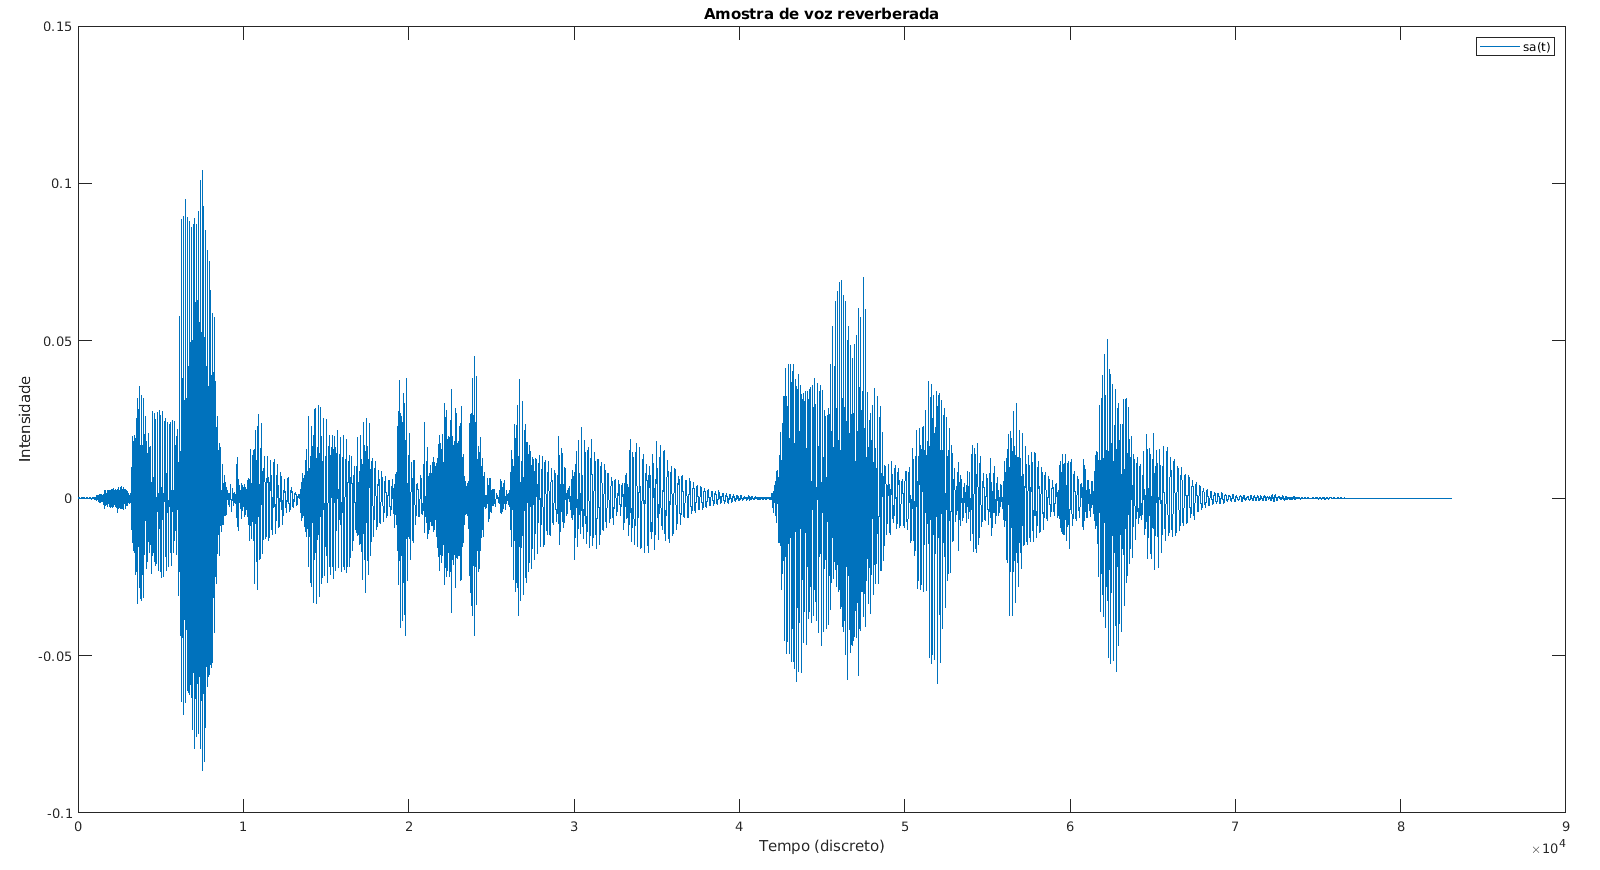
\includegraphics[scale=0.105]{voice-aug-t2.png}
            \end{subfigure}
        \end{figure}
    \end{columns}
\end{frame}

%% ---------------------------------------------------------------------------
% RESULTADOS - AVCD

\begin{frame}{Resultados - AVCD}
    \begin{table} [H]
        \centering
        \begin{tabular}{c|c|c|c|c|c}
    
            \textbf{Exemplo} & 
            \textbf{Sala RIR} & 
            \textbf{Distância (m)} &
            \textbf{AVA} &
            \textbf{SRP} &
            \textbf{SRF} \\
            \hline 
    
            N1 & lecture & 7.1 & M2-T1 & RP-6 & RF-1 \\
            N2 & booth & 1 & H2-T1 & RP-12 & RF-4 \\
            N3 & office & 2 & H1-T1 & RP-4 & RF-4 \\
            N4 & meeting & 1.7 & M1-T2 & RP-11 & RF-2 \\
            N5 & stairway & 1 & H2-T1 & RP-7 & RF-4 \\
    
        \end{tabular}
        \bigbreak
        \bigbreak
        \begin{tabular}{c|c|c|c|c|c}
    
            \textbf{Ex.} & 
            \textbf{$DRR_{org}$ (dB)} & 
            \textbf{$DRR_{res}$ (dB)} & 
            \textbf{$T60_{org}$ (s)} & 
            \textbf{$T60_{res}$ (s)} &
            \textbf{$SNR_{alvo}$} \\
            \hline 
    
            N1 & -4,5 & 17 & 1,38 & 0,56 & 5 \\
            N2 & 4,7 & 17 & 1,01 & 1,39 & 10 \\
            N3 & 0,5 & 14 & 0,75 & 0,60 & 14 \\
            N4 & 6,0 & 16 & 0,81 & 1,16 & 19 \\
            N5 & 5,0 & 18 & 2,70 & 3,68 & 3 \\
    
        \end{tabular}
    \end{table}
\end{frame}

\begin{frame}{Resultados - AVCD}
    \textbf{Experimento empírico}: análise subjetiva de nível de ruído, ordenado de mais para menos ruidoso.
    \vspace{1cm}
    
    \begin{table} [H]
        \centering
        \begin{tabular}{c|c|c}
    
            \textbf{Exemplo} & 
            \textbf{$SNR_{alvo}$ (s)} & 
            \textbf{Ordem} \\
            \hline 
    
            N1 &  5 & 3 \\
            N2 & 10 & 4 \\
            N3 & 14 & 1 \\
            N4 & 19 & 5 \\
            N5 &  3 & 2 \\
    
        \end{tabular}
    \end{table}
\end{frame}

\begin{frame}{Exemplo N4}
    \begin{columns}
        \column{0.5\textwidth}
        \begin{figure}
            \begin{subfigure}{\textwidth}
                \centering
                \textattachfile{audios/voice-og-n4.wav}{\scriptsize amostra de voz original}
                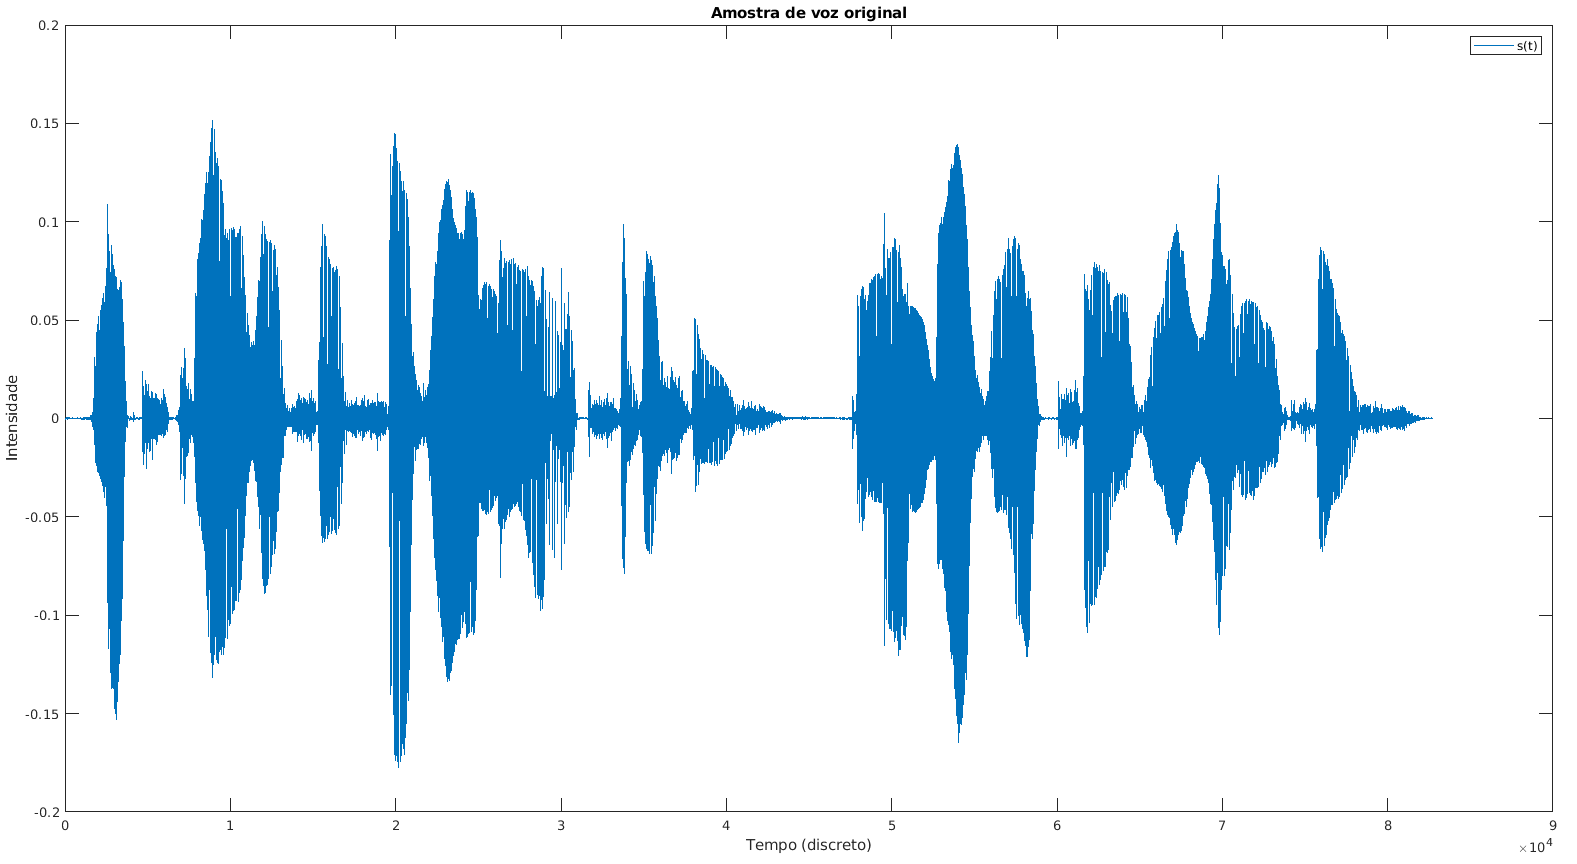
\includegraphics[scale=0.105]{voice-og-n4.png}
            \end{subfigure}
        \end{figure}

        \column{0.5\textwidth}
        \begin{figure}
            \begin{subfigure}{\textwidth}
                \centering
                \textattachfile{audios/voice-aug-n4.wav}{\footnotesize amostra de voz reverberada}
                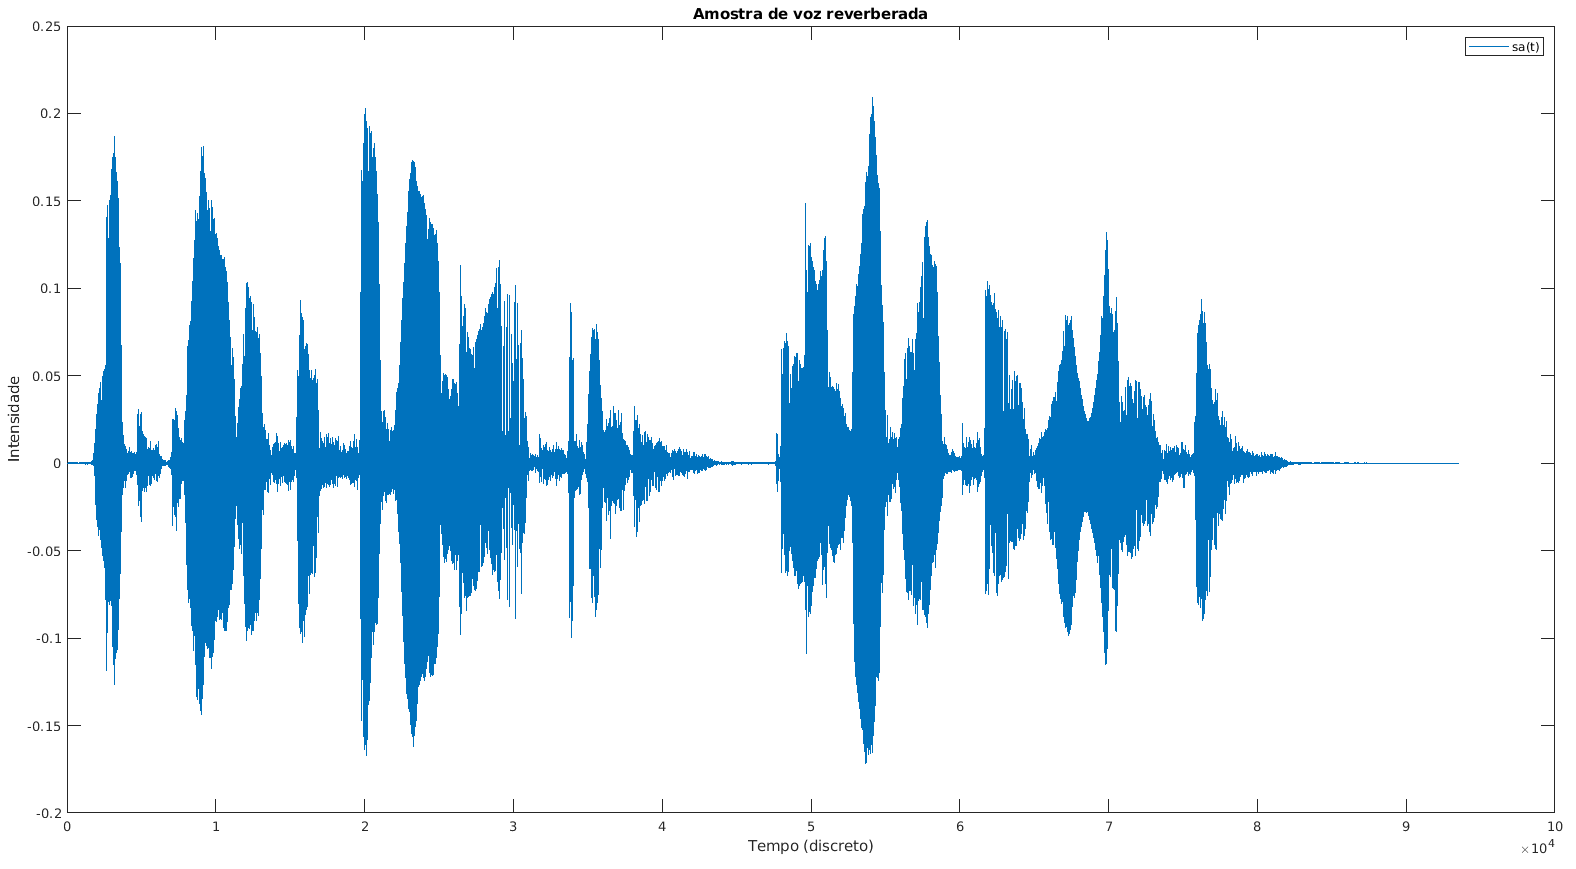
\includegraphics[scale=0.105]{voice-aug-n4.png}
            \end{subfigure}
            \begin{subfigure}{\textwidth}
                \centering
                \textattachfile{audios/voice-ns-n4.wav}{\footnotesize amostra de voz em campo distante}
                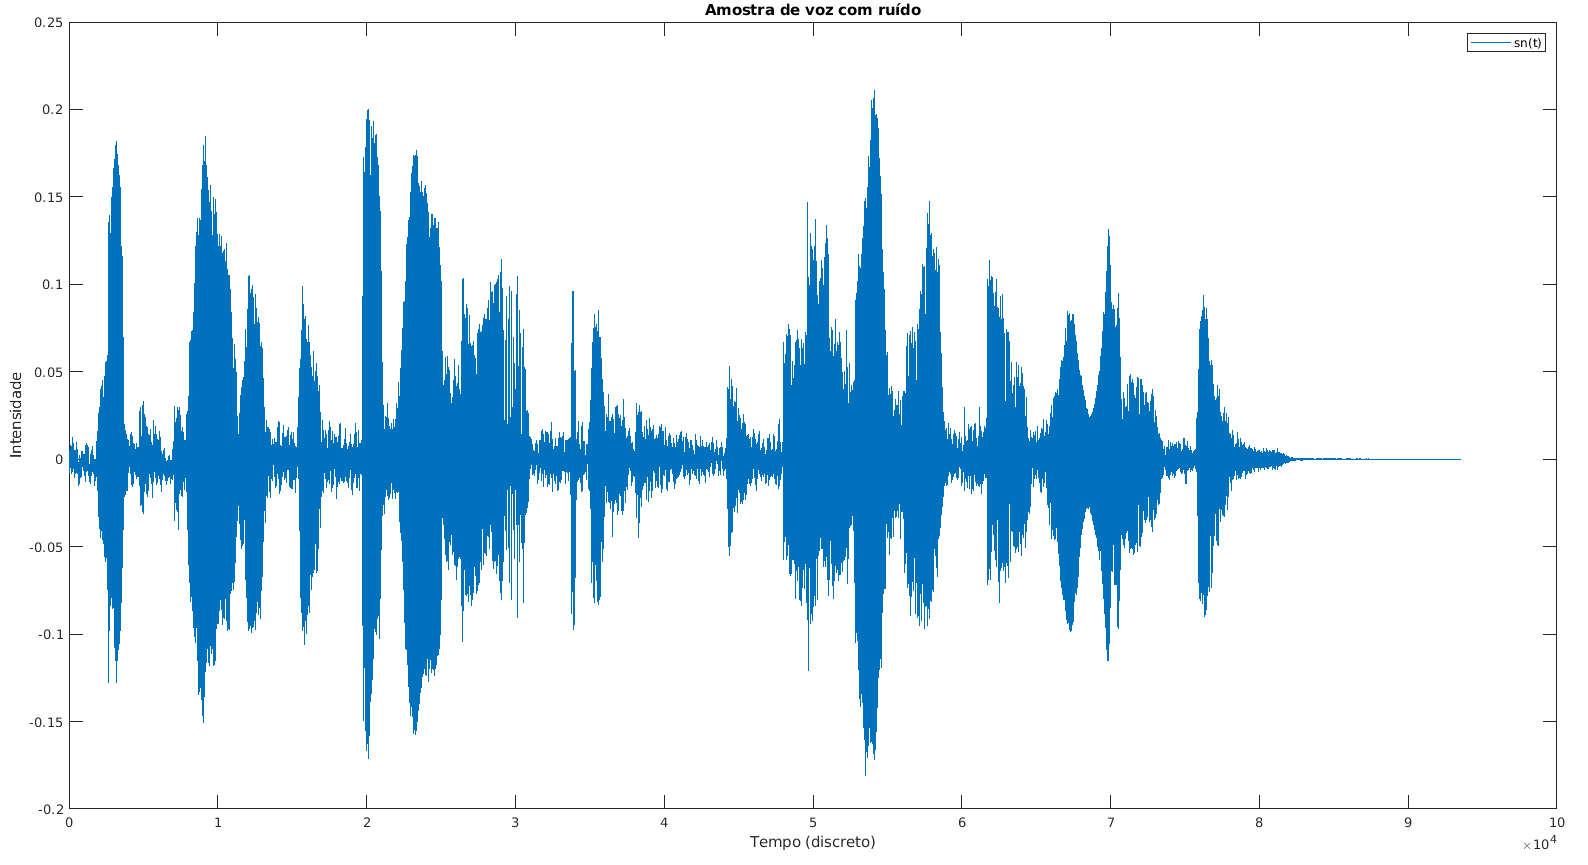
\includegraphics[scale=0.105]{voice-ns-n4.png}
            \end{subfigure}
        \end{figure}
    \end{columns}
\end{frame}

\begin{frame}{Exemplo N5}
    \begin{columns}
        \column{0.5\textwidth}
        \begin{figure}
            \begin{subfigure}{\textwidth}
                \centering
                \textattachfile{audios/voice-og-n5.wav}{\scriptsize amostra de voz original}
                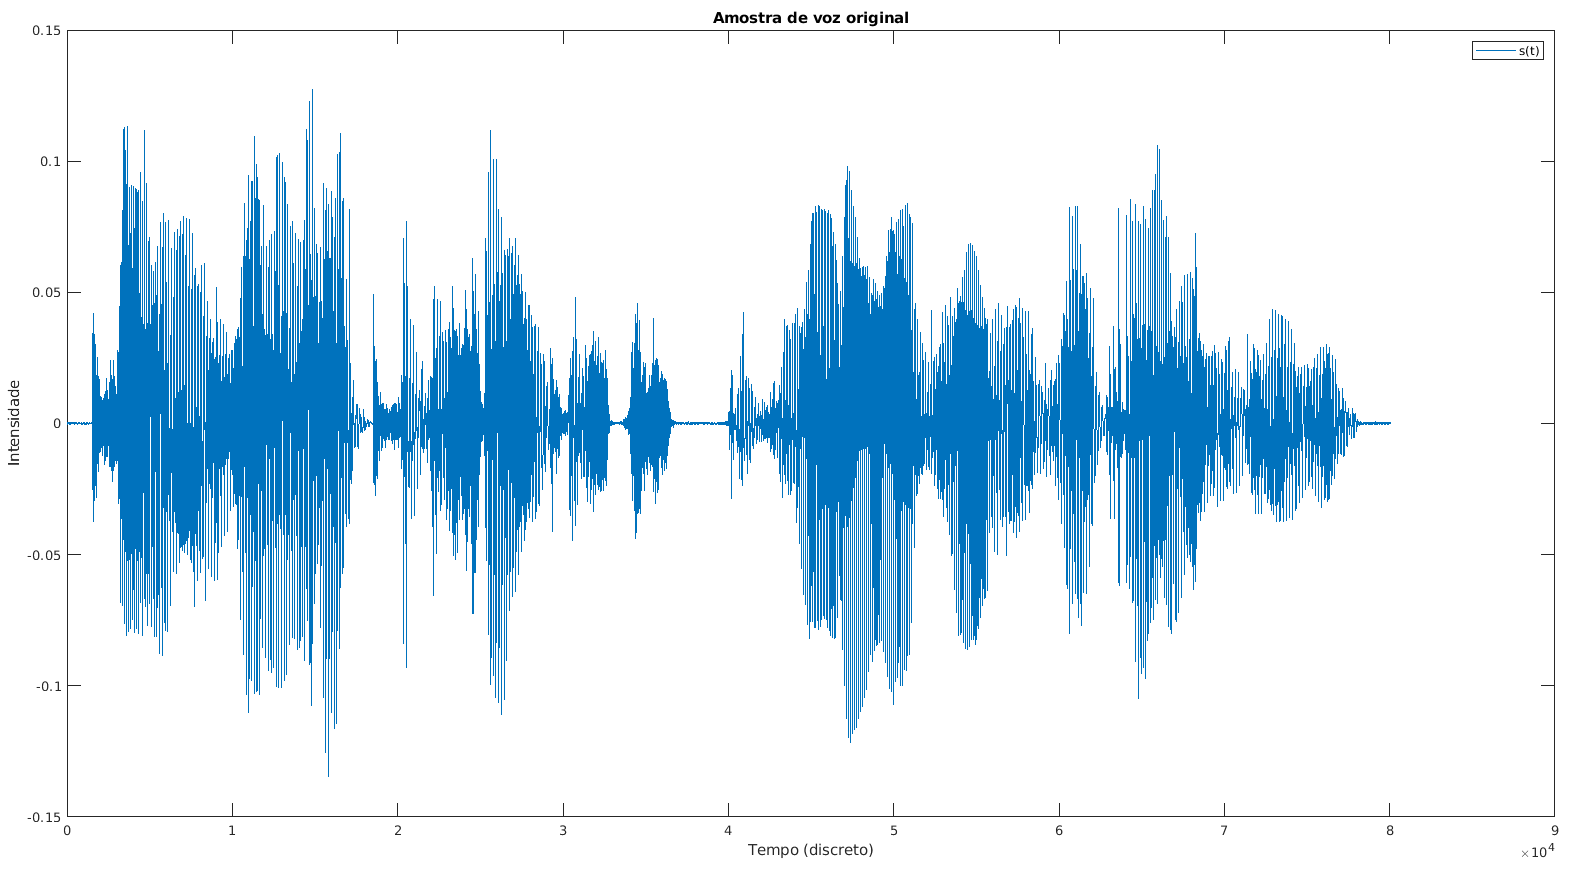
\includegraphics[scale=0.105]{voice-og-n5.png}
            \end{subfigure}
        \end{figure}

        \column{0.5\textwidth}
        \begin{figure}
            \begin{subfigure}{\textwidth}
                \centering
                \textattachfile{audios/voice-aug-n5.wav}{\footnotesize amostra de voz reverberada}
                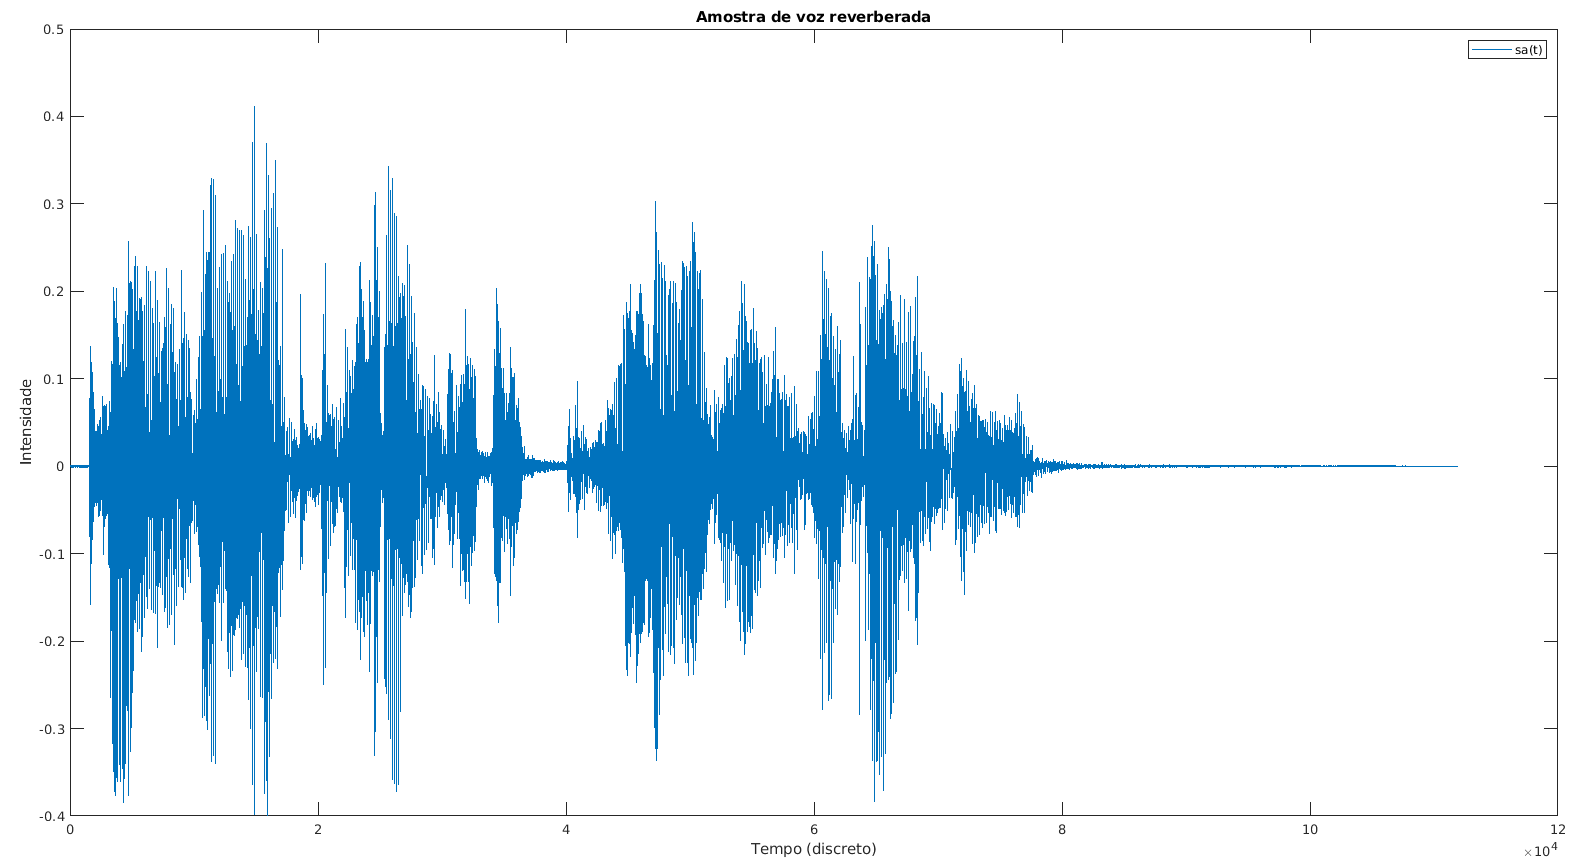
\includegraphics[scale=0.105]{voice-aug-n5.png}
            \end{subfigure}
            \begin{subfigure}{\textwidth}
                \centering
                \textattachfile{audios/voice-ns-n5.wav}{\footnotesize amostra de voz em campo distante}
                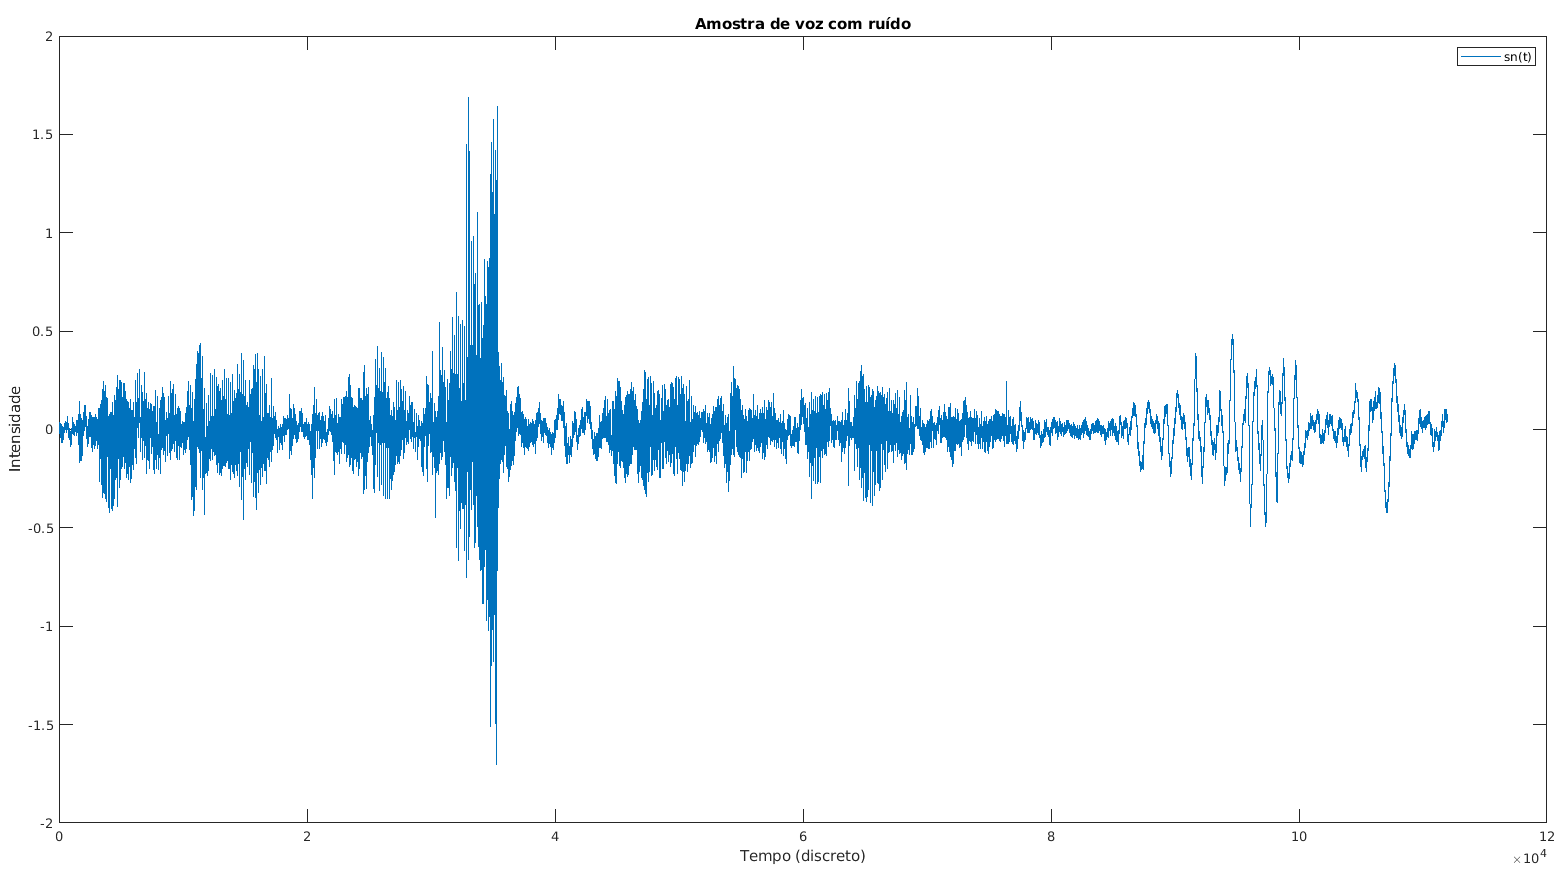
\includegraphics[scale=0.105]{voice-ns-n5.png}
            \end{subfigure}
        \end{figure}
    \end{columns}
\end{frame}